% !TeX spellcheck = en_US
\chapter{Slip and Jump Coefficients}
\label{chap:velocity_slip}
\index{linearized Boltzmann equation}
\index{velocity slip}
\index{temperature jump}


When the Knudsen number is small, rarefaction effects only dominate in the Knudsen layer, hence techniques in the computational fluid dynamics can be used to describe RGD with the velocity-slip and temperature-jump boundary conditions~\citep{sharipov1998data,lockerby2004velocity,leontidis2014numerical}. This chapter is dedicated to the calculation of slip and jump coefficients, as well as the Knudsen layer function, based on the gas kinetic theory.


\section{State of the problem}

A sketch of the slip velocity and Knudsen layer around the planar plate is shown in Fig.~\ref{fig:kramers_dia}. Based on the gas kinetic theory, Maxwell proposed an expression for the slip velocity $u$ at solid surface~\cite{Maxwell1879vii}: 
\begin{equation}\label{eq:slipBC}
u\big|_{x_2=0}=\sigma_P \frac{v_m\mu}{p} \frac{\partial u}{\partial {x_2}}  \bigg|_{x_2=0}+  \sigma_T \frac{\mu}{\rho T} \frac{\partial{T}}{\partial x_3}  \bigg|_{x_2=0},
\end{equation}
where $x_3$ and $x_2$ are respectively the Cartesian coordinates in the parallel
and normal directions to the solid surface; $\sigma_P$ and $\sigma_T$ are respectively the viscous slip coefficient (VSC) and thermal slip coefficient (TSC), which can be determined from the LBE~\citep{ohwada1989numerical,siewert2003viscous,SU2019573} or from experiments~\citep{annis1972thermal,porodnov1978thermal,rojas2015new,Yamaguchi2016JFM}. With the diffuse-specular BC, Maxwell derived
\begin{equation}\label{rough_bc}
\begin{aligned}[b]
\sigma_P=&\frac{2-\alpha_M}{\alpha_M}, \quad
\sigma_T=&\frac{3}{4}.
\end{aligned}
\end{equation}


\begin{figure}[t]
	\centering
	\vskip 0.3cm
	\centering
	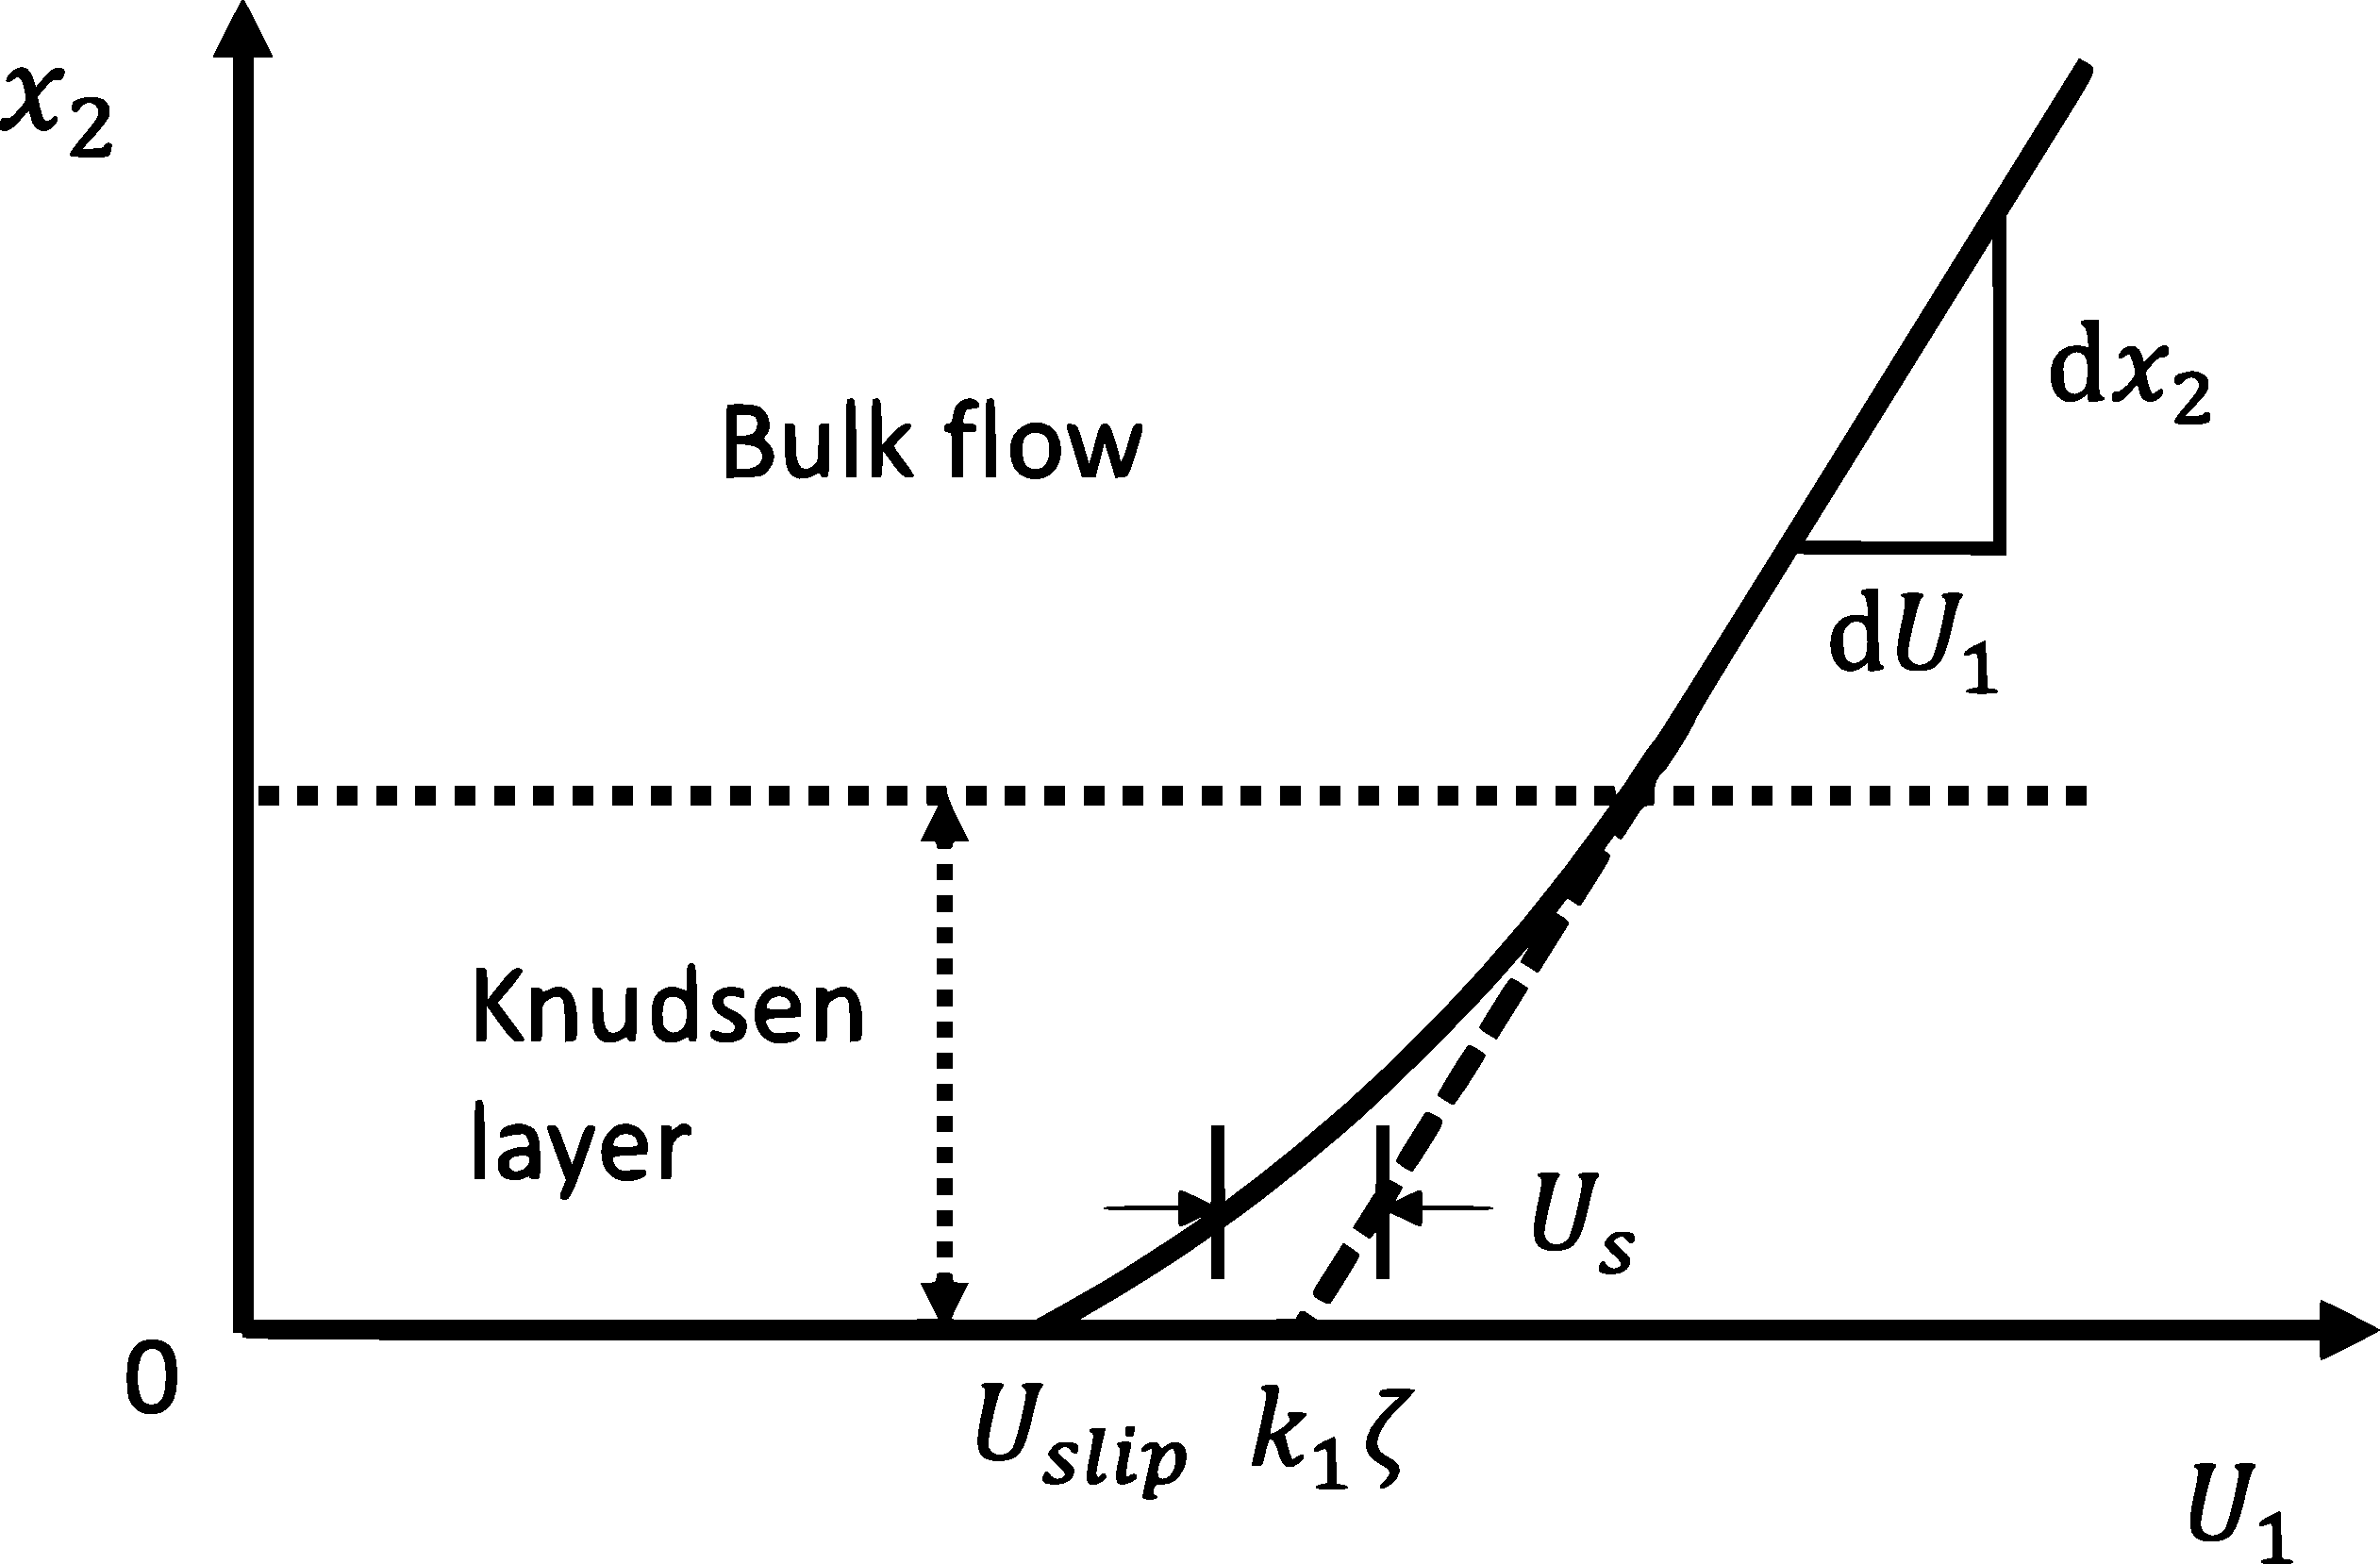
\includegraphics[width=0.4\textwidth]{SlipJump/IMG/kramer}
	\quad
	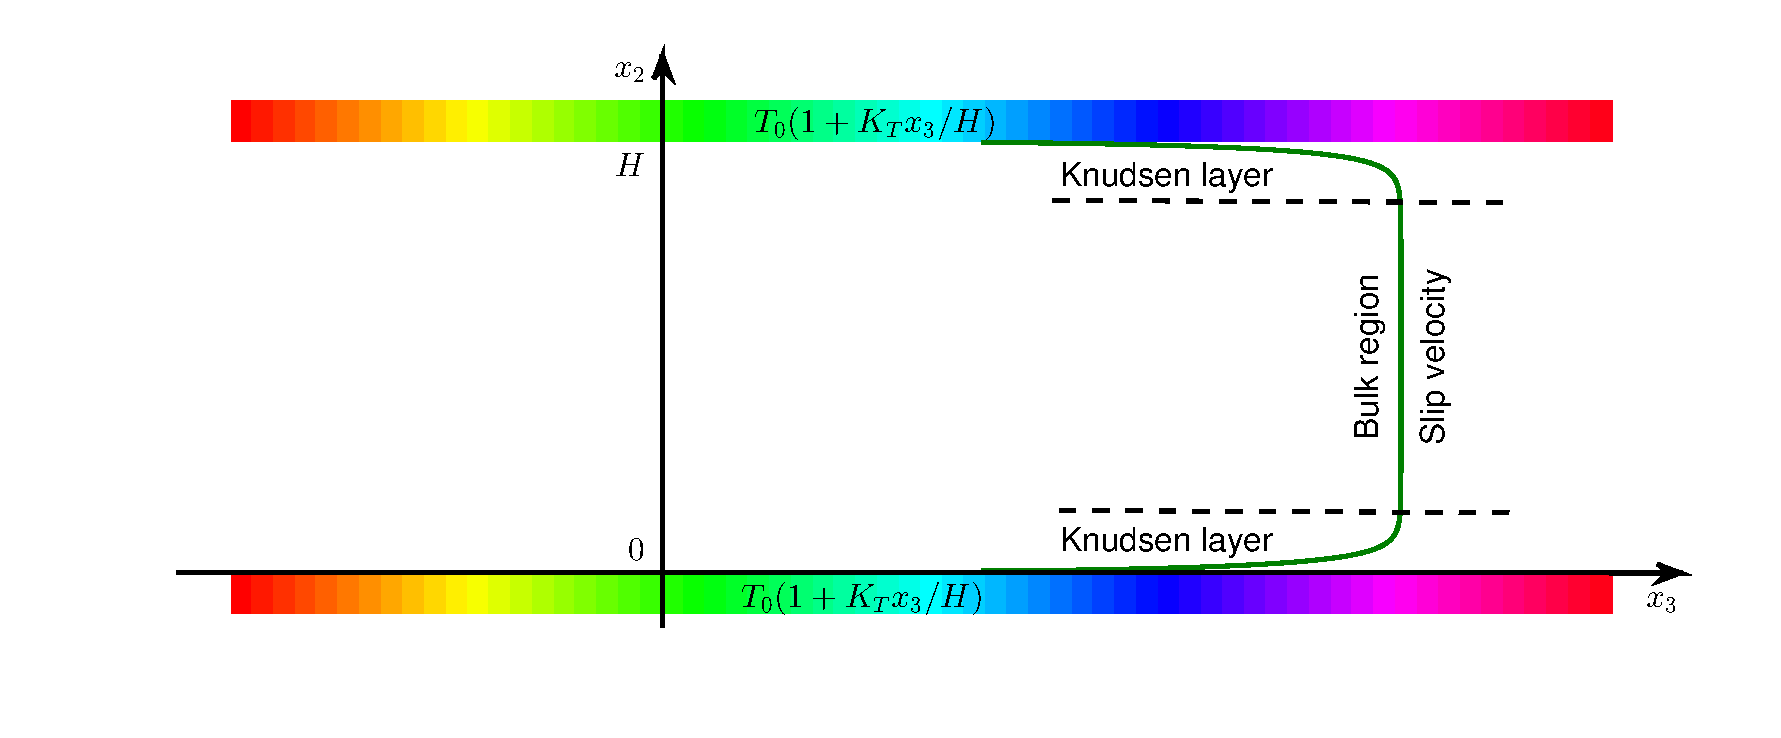
\includegraphics[scale=0.35,viewport=280 50 820 350,clip=true]{SlipJump/IMG/Demo_thermalTranspiration}
%	\\
%	\vskip 0.5cm
%	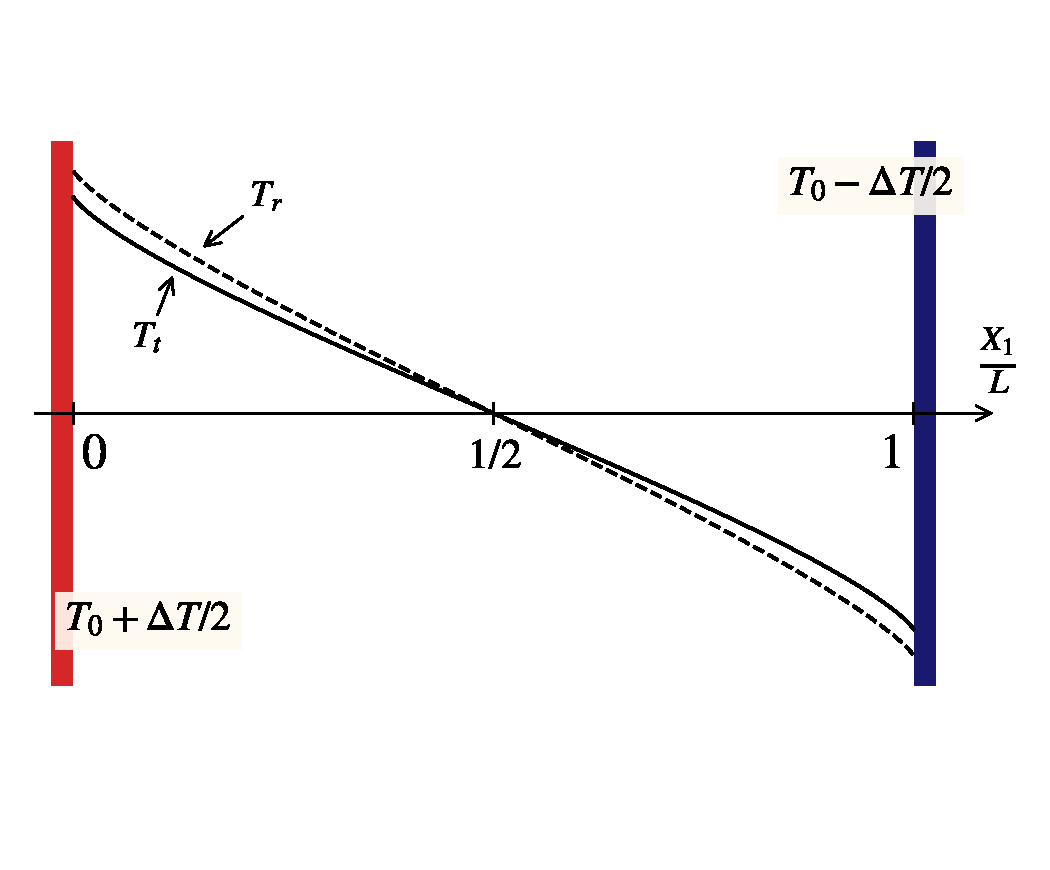
\includegraphics[width=0.4\columnwidth]{SlipJump/IMG/1DFourier_geometry.pdf}%
	\caption{
		(Left) Schematic of the Knudsen layer in Kramer’s problem. The velocity defect (Knudsen layer function) $u_s$ describes the deviation of the linearly extrapolated velocity (dash line) in the bulk region from the true velocity (solid line). %The velocity slope in the bulk region is  $(\text{d}u_1/\text{d}x_2)|_{x_2\rightarrow\infty}=k_1$, the slip length is $\zeta$, while the viscous slip coefficient is defined as $\sigma_P=\zeta/\lambda_e$, where $\lambda_e$ is the equivalent MFP of gas molecules.
	 (Right) Schematic of the thermal transpiration between two parallel plates, where the gas moves from the cold region to the hot region, in spite of the uniform gas pressure. Inside the Knudsen layer, a considerable deviation of the true velocity from the slip velocity in the bulk region is noticed.
  %(Bottom) Schematic of the Knudsen layer and temperature jump in the 1D Fourier flow.
}
	\label{fig:kramers_dia}
\end{figure}




Likewise, the temperature jump at the solid wall is defined as (the schematic is the same as that in Kramer's problem when the velocity is replaced by the temperature)
\begin{equation}\label{Tjump}
T=T_w+\zeta_T\frac{\mu}{p}\sqrt{\frac{2k_BT_w}{m}}\frac{\partial T}{\partial\bm{n}},\quad \text{at wall},
\end{equation}
where $T$ and $T_w$ are the gas temperature and the wall temperature, respectively; $\zeta_T$ is the constant temperature jump coefficient, and $\bm{n}$ is the unit inward normal vector at the wall.
A rough estimation of the coefficient $\zeta_T$ for the diffuse-specular boundary condition is written as~\cite{Kennard1938,Lin1972}
\begin{equation}\label{estimation2}
\zeta_T=\frac{\gamma\sqrt{\pi}}{\left(\gamma+1\right)\text{Pr}}\left(\frac{2-\alpha_M}{\alpha_M}+0.17\right),
\end{equation}
where $\gamma$ is the specific heat ratio of gas. %This estimation is obtained on the assumption that the velocity distribution function of gas molecules does not vary within the Knudsen layer.

%Although one more often deals with molecular gases in practical applications, the above mentioned works only considered monatomic ones. The probably first estimation of temperature jump coefficient was made from the Morse model for gases with only rotations excited that were treated classically~\cite{Lin1972}, read as
%\begin{equation}\label{estimation2}
%\zeta_T=\frac{\gamma\sqrt{\pi}}{\left(\gamma+1\right)\text{Pr}}\left(\frac{2-\alpha_M}{\alpha_M}+0.17\right),
%\end{equation}
%which implies that $\zeta_T$ depends on, considering the physical properties of gases, the internal degrees of freedom (determines the specific heat ratio $\gamma$ and the specific heat $c_p$) and the ratio of the shear viscosity to the thermal conductivity (in the Prandtl number). 

%A more complete analysis about the effects of molecular gases on the velocity slip and temperature jump coefficients as well as the flow properties within the Knudsen layer was recently obtained based on the ES-BGK model~\cite{Hattori2018}. Since the kinetic model contains two adjustable parameters, allowing fitting the experimental values of the shear viscosity, the thermal conductivity, the Prandtl number, and the bulk viscosity (i.e., the second viscosity that is absent in a monatomic gas), the obtained results are also affected by the ratio of the shear and bulk viscosites.

Many problems remain, e.g., (i) why the TSC is not a function of TMAC and (ii) how does the intermolecular potential and internal structure of molecular gases affect the slip and jump coefficients, are not addressed. This chapter is dedicated to answering these questions. 





%\section{ Near wall scaling law of the constitution and slip BC}
%
%
%The VSC and KLF can be used to incorporate the rarefaction effects into the hydrodynamic equations, which can be realized by constructing the near wall scaling law of the constitution and the slip BC~\cite{lockerby2005capturing,guo2007extended}.



%\subsection{Near wall scaling constitutions}
%
%
%For linearized Couette flow, we know that the macroscopic velocity satisfies Eq.~\eqref{synthetic}, where the rarefaction effects are contained in the high-order terms. A simple way to take these terms into account in the Navier-Stokes level is to introduce the effect viscosity $\mu_e$ (and hence effective rarefaction parameter $\delta_{rp}_e$), so that Eq.~\eqref{synthetic} becomes ${\partial {u_1} }/{\partial{}x_2}=-\delta_e{P_{12}}$. Thus, the ratio between the effective viscosity, which is a function to the wall distance, to the real viscosity, can be calculated as follows:
%\begin{equation}\label{eq:numerical_vis}
%\frac{\mu_e}{\mu}=-\delta P_{12}\left(\frac{du_1}{dx_2}\right)^{-1}.
%\end{equation}
%
%
%Alternatively, when the KLF is known, \cite{lockerby2005capturing} proposed the following effective viscosity:
%\begin{equation}\label{eq:pre_vis}
%\frac{\mu_e}{\mu}=\frac{1}{1-\varPsi(\tilde{x}_2)},
%\end{equation}
%where $\tilde{x}_2=x_2/\lambda$, and $	\varPsi(\tilde{x}_2)=du_s\left(\tilde{x}_2\right)/d\tilde{x}_2$ is defined by differentiating the Knudsen layer function Eq.~\eqref{eq:vel_fit} with $M=N=2$ with respect to $\tilde{x}_2$, i.e.,
%\begin{equation}\label{eq:vel_grad}
%\frac{du_s(\tilde{x}_2)}{d\tilde{x}_2}=\sum_{n=0}^{2}\sum_{m=0}^{2}c_{n,m}\tilde{x}_2^{m+n-1}\left(\ln\tilde{x}_2\right)^{m-1}\left[(m+n)\ln\tilde{x}_2+m\right].
%\end{equation}
%Note that for a moderate value of $\delta_{rp}$, the KLFs near the two solid surface start to interference, and Eq.~\eqref{eq:pre_vis} should be corrected as~\cite{lockerby2008modelling}
%\begin{equation}\label{effective}
%\frac{\mu_e}{\mu}=\left[1-\varPsi(\tilde{x}_2)-\varPsi\left(\frac{1}{Kn}-\tilde{x}_2\right)\right]^{-1}.
%\end{equation}
%
%% Eq.~\eqref{eq:vel_grad} with the fitting coefficients in tables~\ref{table_df_coe} and~\ref{table_cl_coe}
%%is accurate for $x_2\leq 3\lambda$, at which for a less rarefied gas flow $\delta_{rp}>1$ confined by two parallel plates, the relative deviation of velocity predicted by the Knudsen layer function Eq.~\eqref{eq:vel_fit} and the Navier-Stokes equations is less than $1\%$. Therefore the viscosity beyond this distance is equal to the real gas one of the bulk flow.  In addition, for a moderate rarefied gas flow, the Knudsen layers near both plates have an  the interference with each other, in which
%
%
%Figure~\ref{fig:effective_vis} shows the ratio of the effective viscosity $\mu_e$ to the real viscosity $\mu$ of the gas in Couette flow of different rarefaction parameters. It is found that, with the accurate profile of KLF, \eqref{effective} predicts effective viscosity in good agreement with those from the numerical solution of the LBE, for $\delta_{rp}$ down to 0.1. However, if we use the KLF as in Eq.~\eqref{eq:loc_vis}, although it works for $\delta_{rp}=100$, it gradually lose accuracy when $\delta_{rp}$ decreases. It is worth noting that  KLFs developed by~\cite{lockerby2005usefulness} which decay exponentially from the way show even worse prediction of the effective viscosity.
%
%%
%% when $\delta_{rp}\geq 1$, Eq.~\eqref{eq:pre_vis} can accurately reproduce the viscosity given by Eq.~\eqref{eq:numerical_vis}; and even for $\delta_{rp}=10$, the maximum relative difference is still less than $10\%$. We also notice that when $\delta_{rp}=100$, the effective viscosity derived based on Eq.~\eqref{eq:loc_vis} agrees well with that from Eq.~\eqref{eq:numerical_vis}, while the deviation becomes visible as the decrease of $\delta_{rp}$; eventually, when $\delta_{rp}\geq1$, \eqref{eq:loc_vis} can not even give a reasonable solution of the effective viscosity.
%
%
%%
%\begin{figure}
%	\begin{centering}
%		\includegraphics[width=0.6\textwidth]{effective_vis.eps}
%		\par\end{centering}
%	\caption{The ratio between the effective viscosity $\mu_e$ and real viscosity $\mu$ of the HS gas, in the linearized Couette flow between two parallel plates, with the diffuse BC. Due to symmetry, only half of the spatial domain is shown. Solid lines are computed from Eq.~\eqref{eq:numerical_vis} using the numerical results from the LBE; symbols are calculated  by Eq.~\eqref{eq:pre_vis} using the KLF; dash lines are the numerical results according to Eq.~\eqref{eq:loc_vis} given by~\cite{lockerby2005capturing}. }
%	\label{fig:effective_vis}
%\end{figure}
%%
%\subsection{Slip BC}\label{sec:slip_bounary}
%From Eq.~\eqref{NS_fit} and Eq.~\eqref{slip_coe}, the slip velocity $u_{slip}$ on the boundary can be written as
%\begin{equation}\label{slip_boun}
%u_{slip}=k_1\lambda\left[\sigma_P+u_s(\tilde{x}_2=0)\right],
%\end{equation}
% The VSC $\sigma_P$ and the defect velocity on the boundary $u_s(\tilde{x}_2=0)$ can be determined according to Eq.~\eqref{CL_fit} and the KLF Eq.~\eqref{eq:vel_fit}.
%
%Therefore, the slip velocity Eq.~\eqref{slip_boun} on the boundary and the effective viscosity Eq.~\eqref{eq:pre_vis} near the wall can be used within the computational fluid dynamics frame to imitate the micro-and nanoscale flows.
%


\section{Thermal slip}
\index{thermal slip coefficient}
\index{thermal transpiration}



The GSIS is applied to find the steady-state solution of thermal transpiration~\cite{Wang2020PoF,Su2021CMAME}. When the steady-state solution is obtained, the KLF, which is the defect velocity $u_d$ inside the Knudsen layer, is calculated according to the following equation:
\begin{equation}
u_d\left(\frac{x_2}{\text{Kn}}\right)=\frac{1}{\text{Kn}}\left[u_3\left(\frac{1}{2}\right)-u_3(x_2)\right].
\end{equation} 
Meanwhile, the TSC is calculated as
\begin{equation}
\sigma_T=2\delta_{rp}u_3\left(\frac{1}{2}\right).
\end{equation}



%When the steady-state solution is obtained,  the KLF, which is the defect velocity $u_d$ inside the Knudsen layer, is calculated according to the following equation (see Fig.~\ref{Demo}):
%\begin{equation}\label{NS_fit}
%u_d\left(\frac{x_2}{Kn}\right)=\frac{1}{Kn}\left[u_3\left(\frac{1}{2}\right)-u_3(x_2)\right],
%\end{equation}
%where the Knudsen number is formally defined as $\text{Kn}=\lambda/H=\sqrt{\pi}/2\delta_{rp}$. 
%Meanwhile, the TSC is calculated as
%\begin{equation}\label{slip_coe}
%\sigma_T=2\delta_{rp}u_3\left(\frac{1}{2}\right).
%\end{equation}


%We find that $\delta_{rp}_{rp}=100$ is accurate enough to recover the KLF and TSC, when compared to the solution of $\delta_{rp}_{rp}=1000$. By contrast, when $\delta_{rp}_{rp}=10$, two Knudsen layers interact with each other, which leads to an inaccurate KLF.

\begin{table}[t]
	\centering
	\caption{\label{table_CL}TSCs  for HS, Maxwellian and VHS ($\omega=1.5$) molecules under the Cercignani-Lampis  BC  with different values of TMAC and EAC.}
		\begin{tabular}{lccccr}
			\hline
			$\alpha_t$  & $\omega$
			&  $\alpha_n=0.25$ & $ \alpha_n=0.5$  &    $\alpha_n=0.75$ &    $\alpha_n= 1$\\
			%%  \rowcolor[gray]{.9}
			$0.25$
			& 0.5   & 0.878961  & 0.939289   & 0.997097 &  1.052749  \\
			&1.0    & 0.957507  & 1.031589   & 1.103622 &  1.173821  \\
			&1.5    & 1.073727  & 1.166016   & 1.256071 &  1.343934  \\
			%   \rowcolor[gray]{.9}
			$0.5$
			& 0.5   & 0.915032   & 0.953837   & 0.99152 & 1.028174  \\
			&1.0    & 1.038391   & 1.085497   & 1.132079 & 1.178087  \\
			&1.5    & 1.207714   & 1.265554   & 1.323069 &  1.380077  \\
			
			$0.75$
			& 0.5   & 0.963946   & 0.982787   & 1.001310  & 1.019504 \\
			&1.0    & 1.111326   & 1.134018   & 1.156801  & 1.179587\\
			&1.5    & 1.309165   & 1.336765   & 1.364675 & 1.392753  \\
			%   \rowcolor[gray]{.9}
			$1.0$
			& 0.5   & 1.018280   & 1.018280   & 1.018280 & 1.018280 \\
			&1.0    & 1.179794   & 1.179794   & 1.179794 & 1.179794 \\
			&1.5    & 1.394533   & 1.394533   & 1.394533 & 1.394533  \\
			
			%   \rowcolor[gray]{.9}
			$1.25$
			& 0.5   & 1.070999   & 1.053104   & 1.035091 &  1.017060 \\
			&1.0    & 1.245767   & 1.224484   & 1.202513  & 1.180003 \\
			&1.5    & 1.476314   & 1.450674   &1.423957 &  1.396309  \\
			
			%   \rowcolor[gray]{.9}
			$1.5$
			& 0.5   & 1.114835   & 1.079992   & 1.044506 & 1.008646 \\
			&1.0    & 1.310156   & 1.269058   & 1.226052 & 1.181462 \\
			&1.5    & 1.564814   & 1.515439   & 1.463286 & 1.408579  \\
			
			%   \rowcolor[gray]{.9}
			$1.75$
			& 0.5   & 1.142984   & 1.092304   & 1.040058   & 0.986740\\
			&1.0    & 1.372910   & 1.313785   & 1.251073   & 1.185256 \\
			&1.5    & 1.667706   & 1.596793   & 1.520959   &  1.440373  \\
			
			$2$
			& 0.5   & 1.150836   & 1.085729   &1.017732 & 0.947616\\
			&1.0    & 1.433179   & 1.358215   &1.277626  &1.191998 \\
			&1.5    & 1.788740   & 1.698623   &1.601268 &  1.496587\\
			\hline 
		\end{tabular}
\end{table}




\subsection{Thermal slip coefficient}

Very little data of TSC has been obtained from the LBE~\cite{wakabayashi1996numerical,siewert2003linearized}, particularly the TSCs for different  intermolecular potentials. Here, we close this gap by solving the LBE via SIS, for different intermolecular potentials and gas-surface interactions.

\begin{figure}
	\centering
	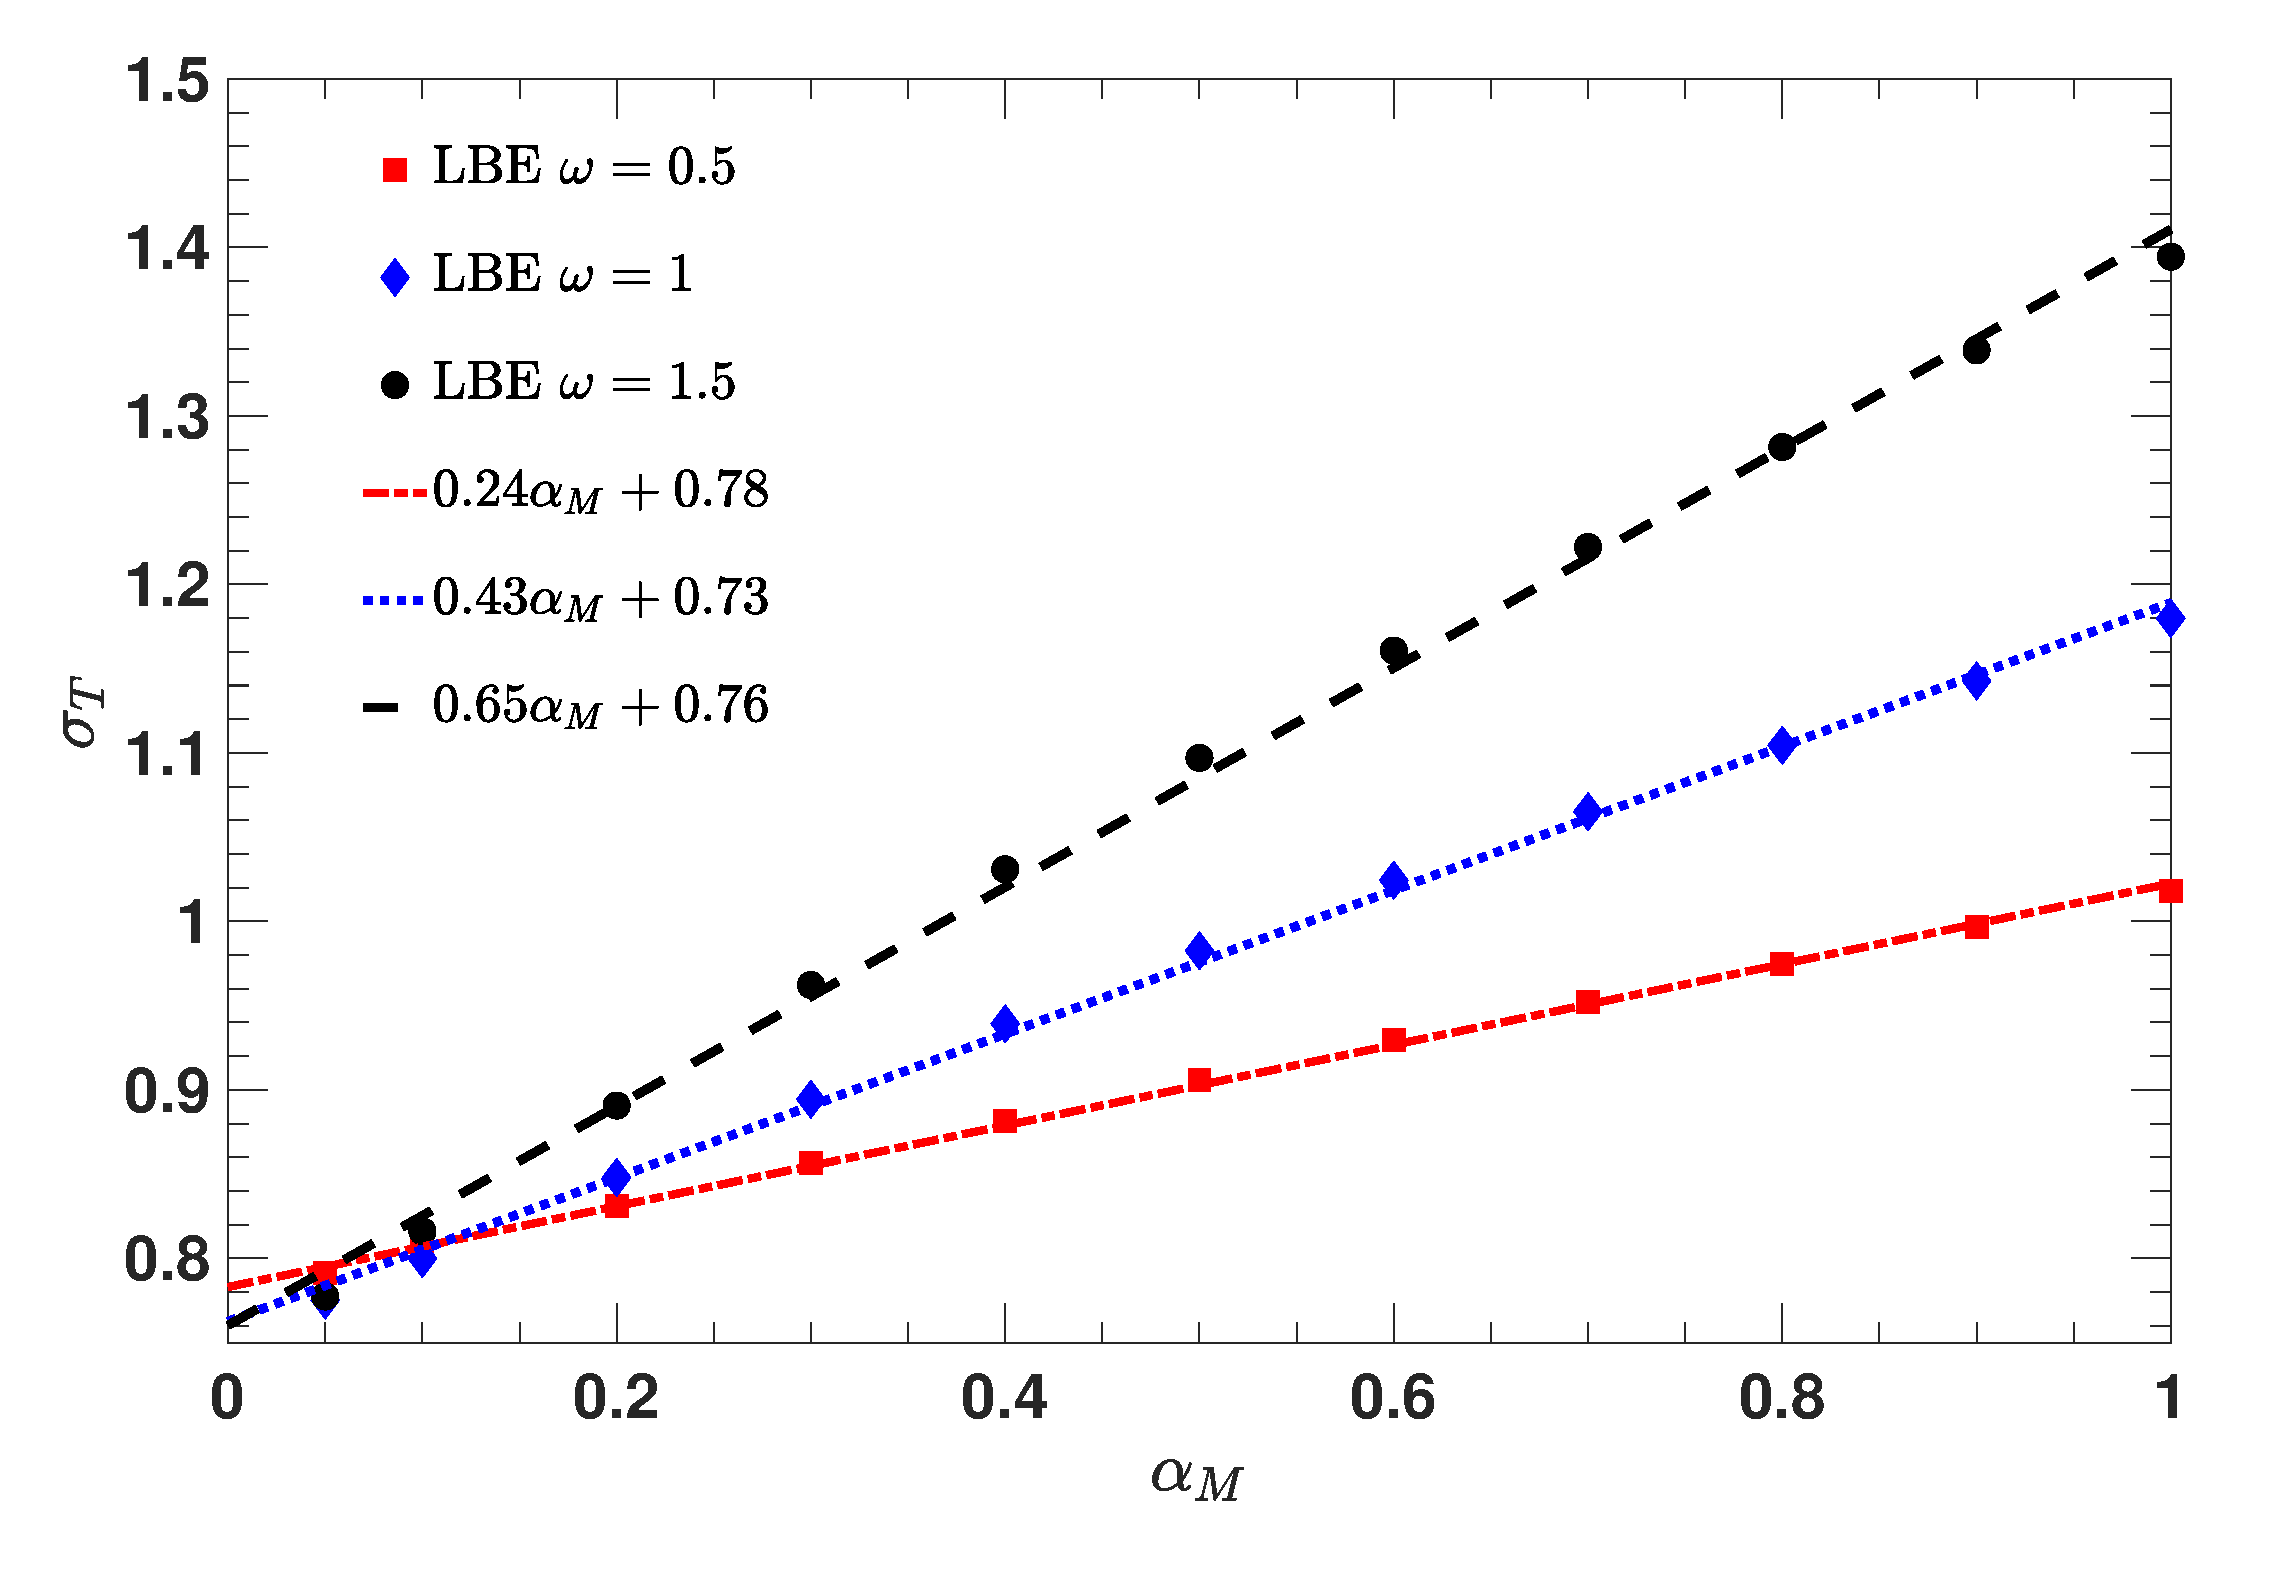
\includegraphics[width=0.6\textwidth]{SlipJump/IMG/ThermalCoe_MaxBound}
	\caption{Symbols: TSCs obtained from the LBE for HS, Maxwellian, and variable hard sphere (VHS, $\omega=1.5$) molecules, when the diffuse-specular BC is used. Lines: linear fittings of TSCs with respect to the TMAC. }
	\label{fig:TSC_Bound0}
\end{figure}

%We first solve the LBE for HS molecules with the diffuse-specular BC and compare the TSC with those obtained by Wakabayashi~\cite{wakabayashi1996numerical} and Siewert~\cite{siewert2003linearized}. We find that the three groups of data agree well with each other, especially the relative difference between our results and those of Siewert~\cite{siewert2003linearized} is less than $10^{-3}$; this confirms the accuracy of our method. 


Figure~\ref{fig:TSC_Bound0} shows the TSC in the diffuse-specular BC. When $\alpha_M$ is fixed, in most cases the TSC increases with the viscosity index, except that this trend is reversed when $\alpha_M$ approaches zero. When the intermolecular potential is fixed, we find that the data obtained from the LBE can be approximately fitted by linear functions of $\alpha_M$, with the relative discrepancy between fitting results and numerical data being less than $1.5\%$; and the slope of fitting increases with the viscosity index. %This linear change of TSC with the TMAC is consistent with the results obtained from the kinetic model equation~\citep{SharipovData2011}. 





\begin{figure}[t]
	\centering
	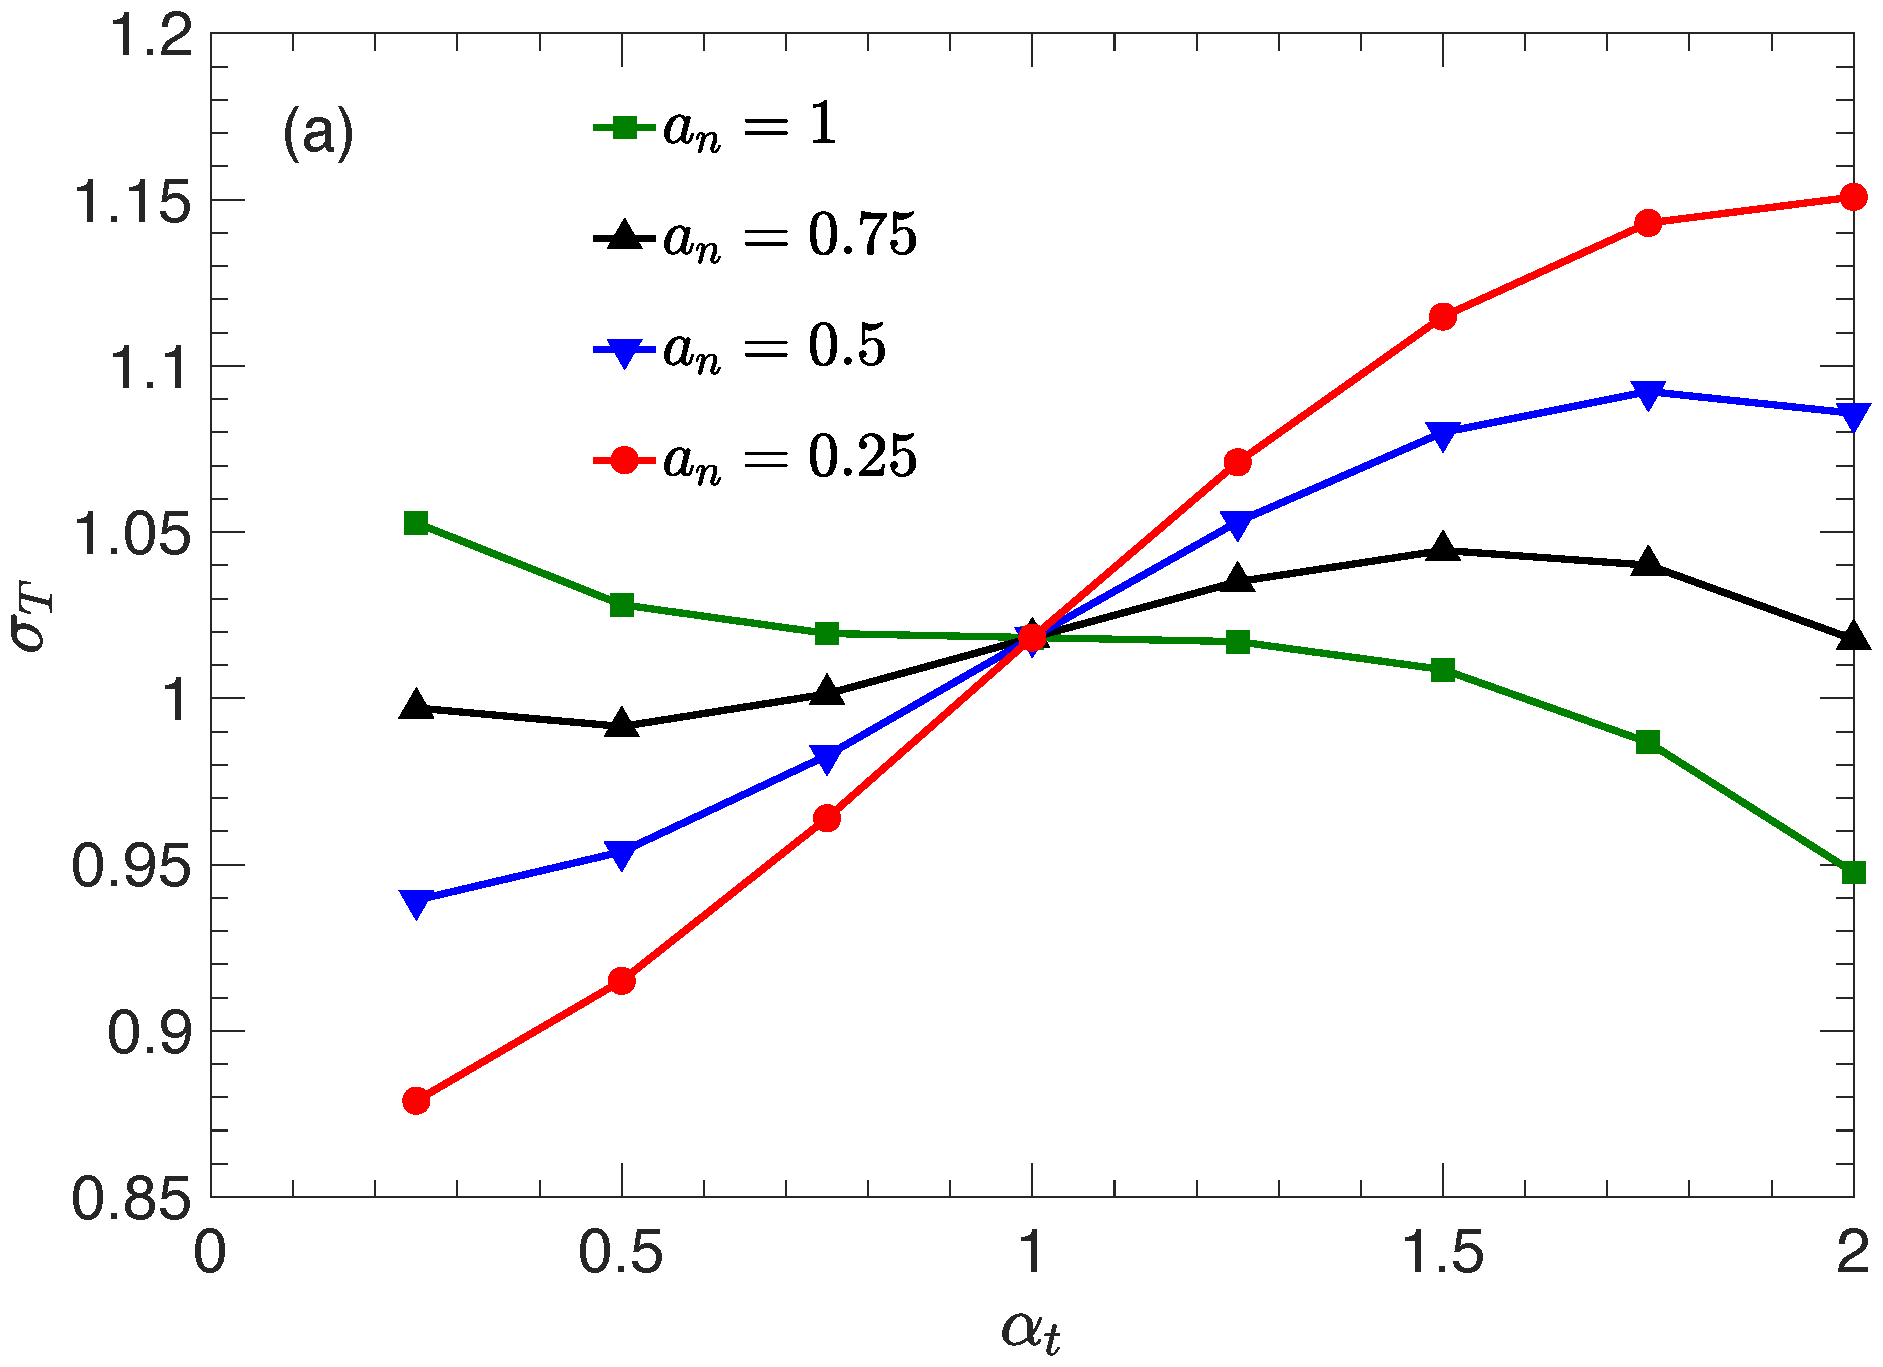
\includegraphics[width=0.45\textwidth]{SlipJump/IMG/TSC_vs_TMAC_Omega05}\
	\hskip 15pt
	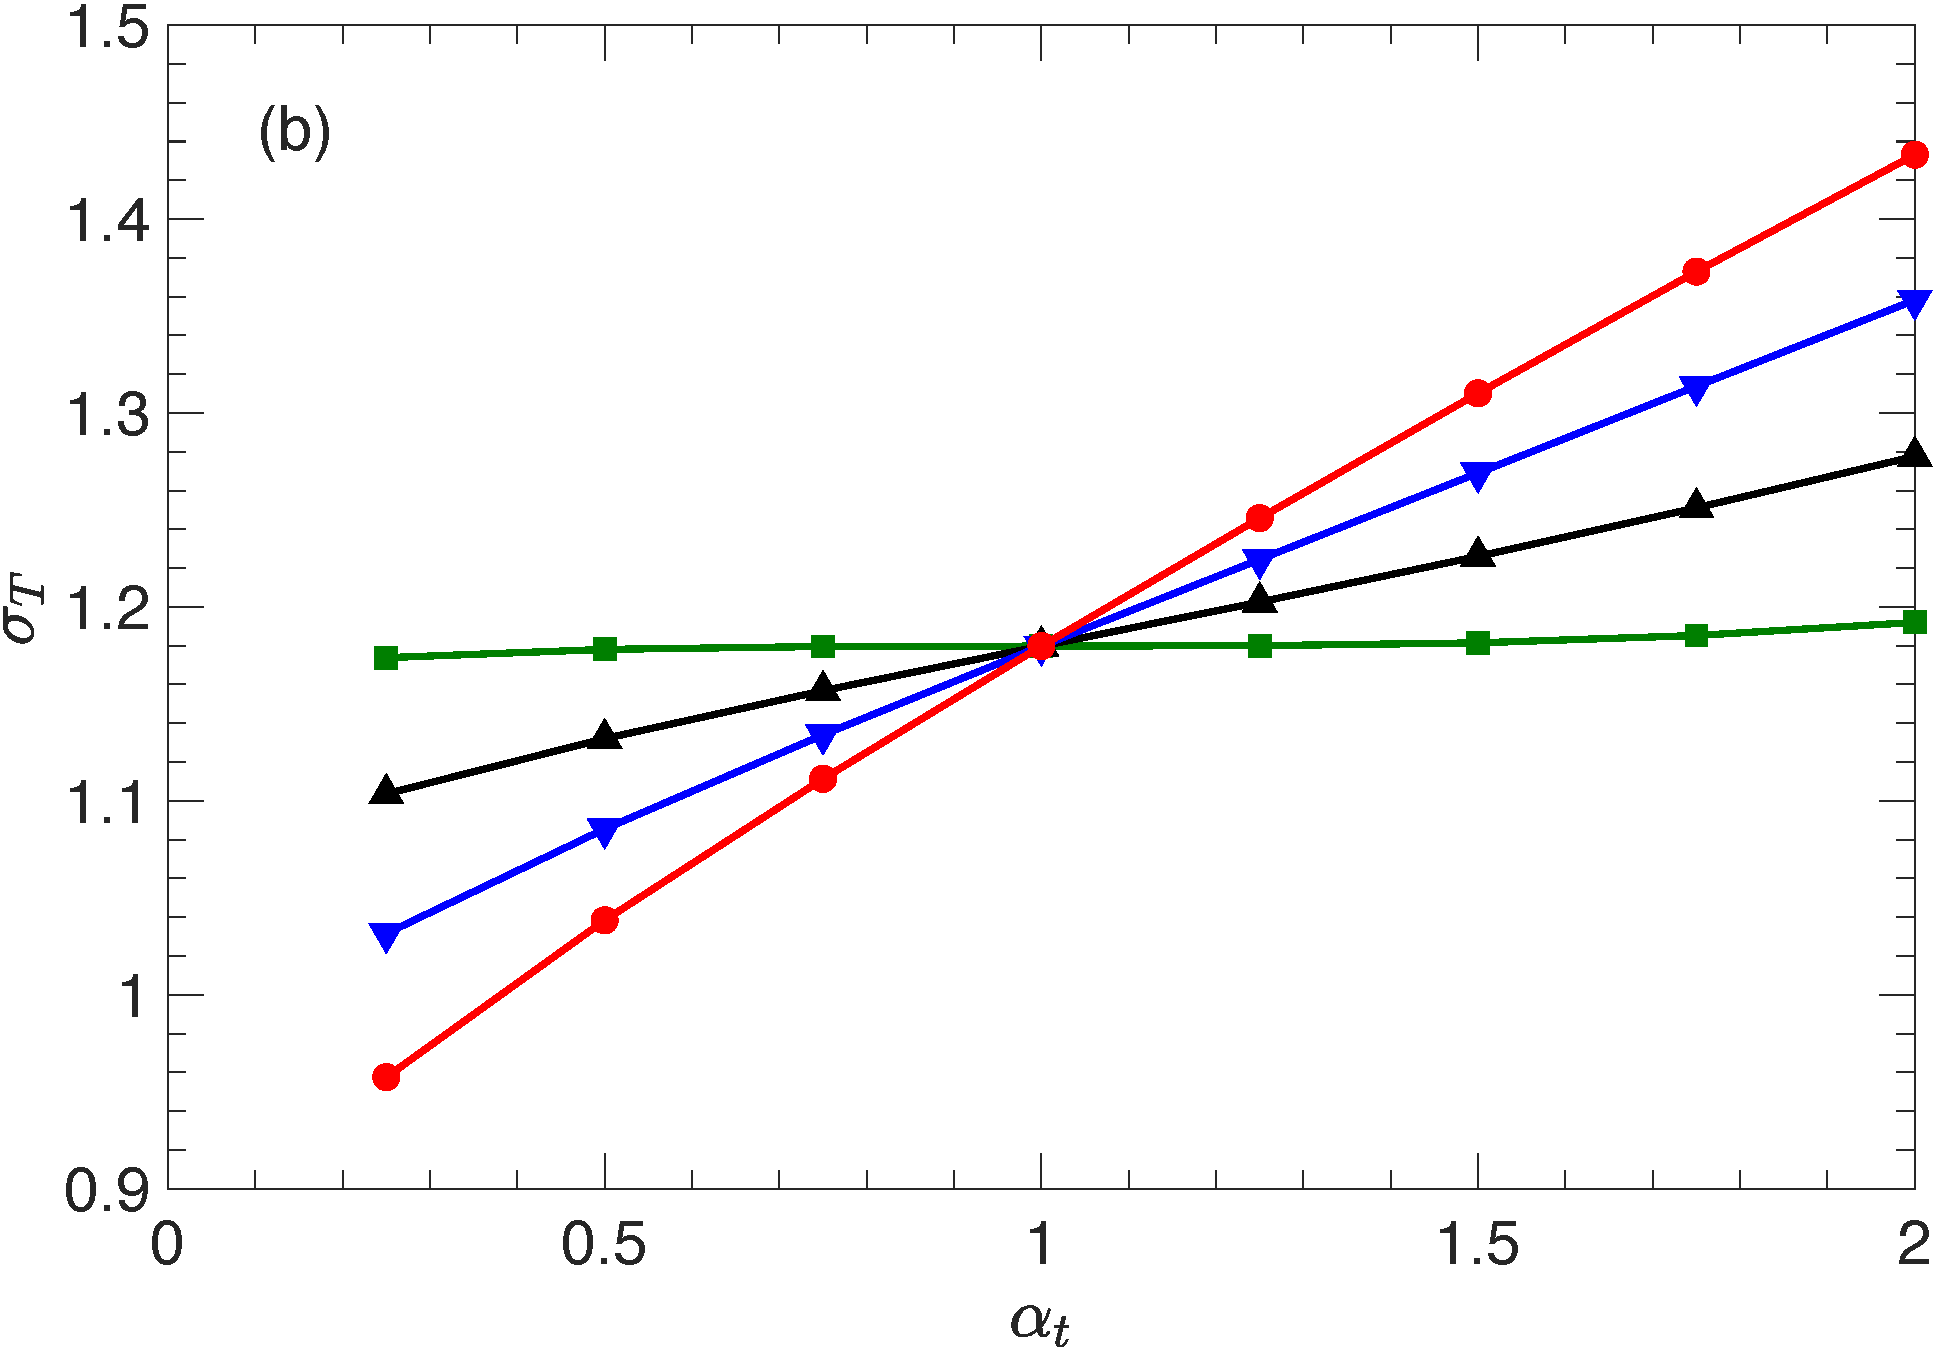
\includegraphics[width=0.45\textwidth]{SlipJump/IMG/TSC_vs_TMAC_Omega1}\\
	\vskip 10pt
	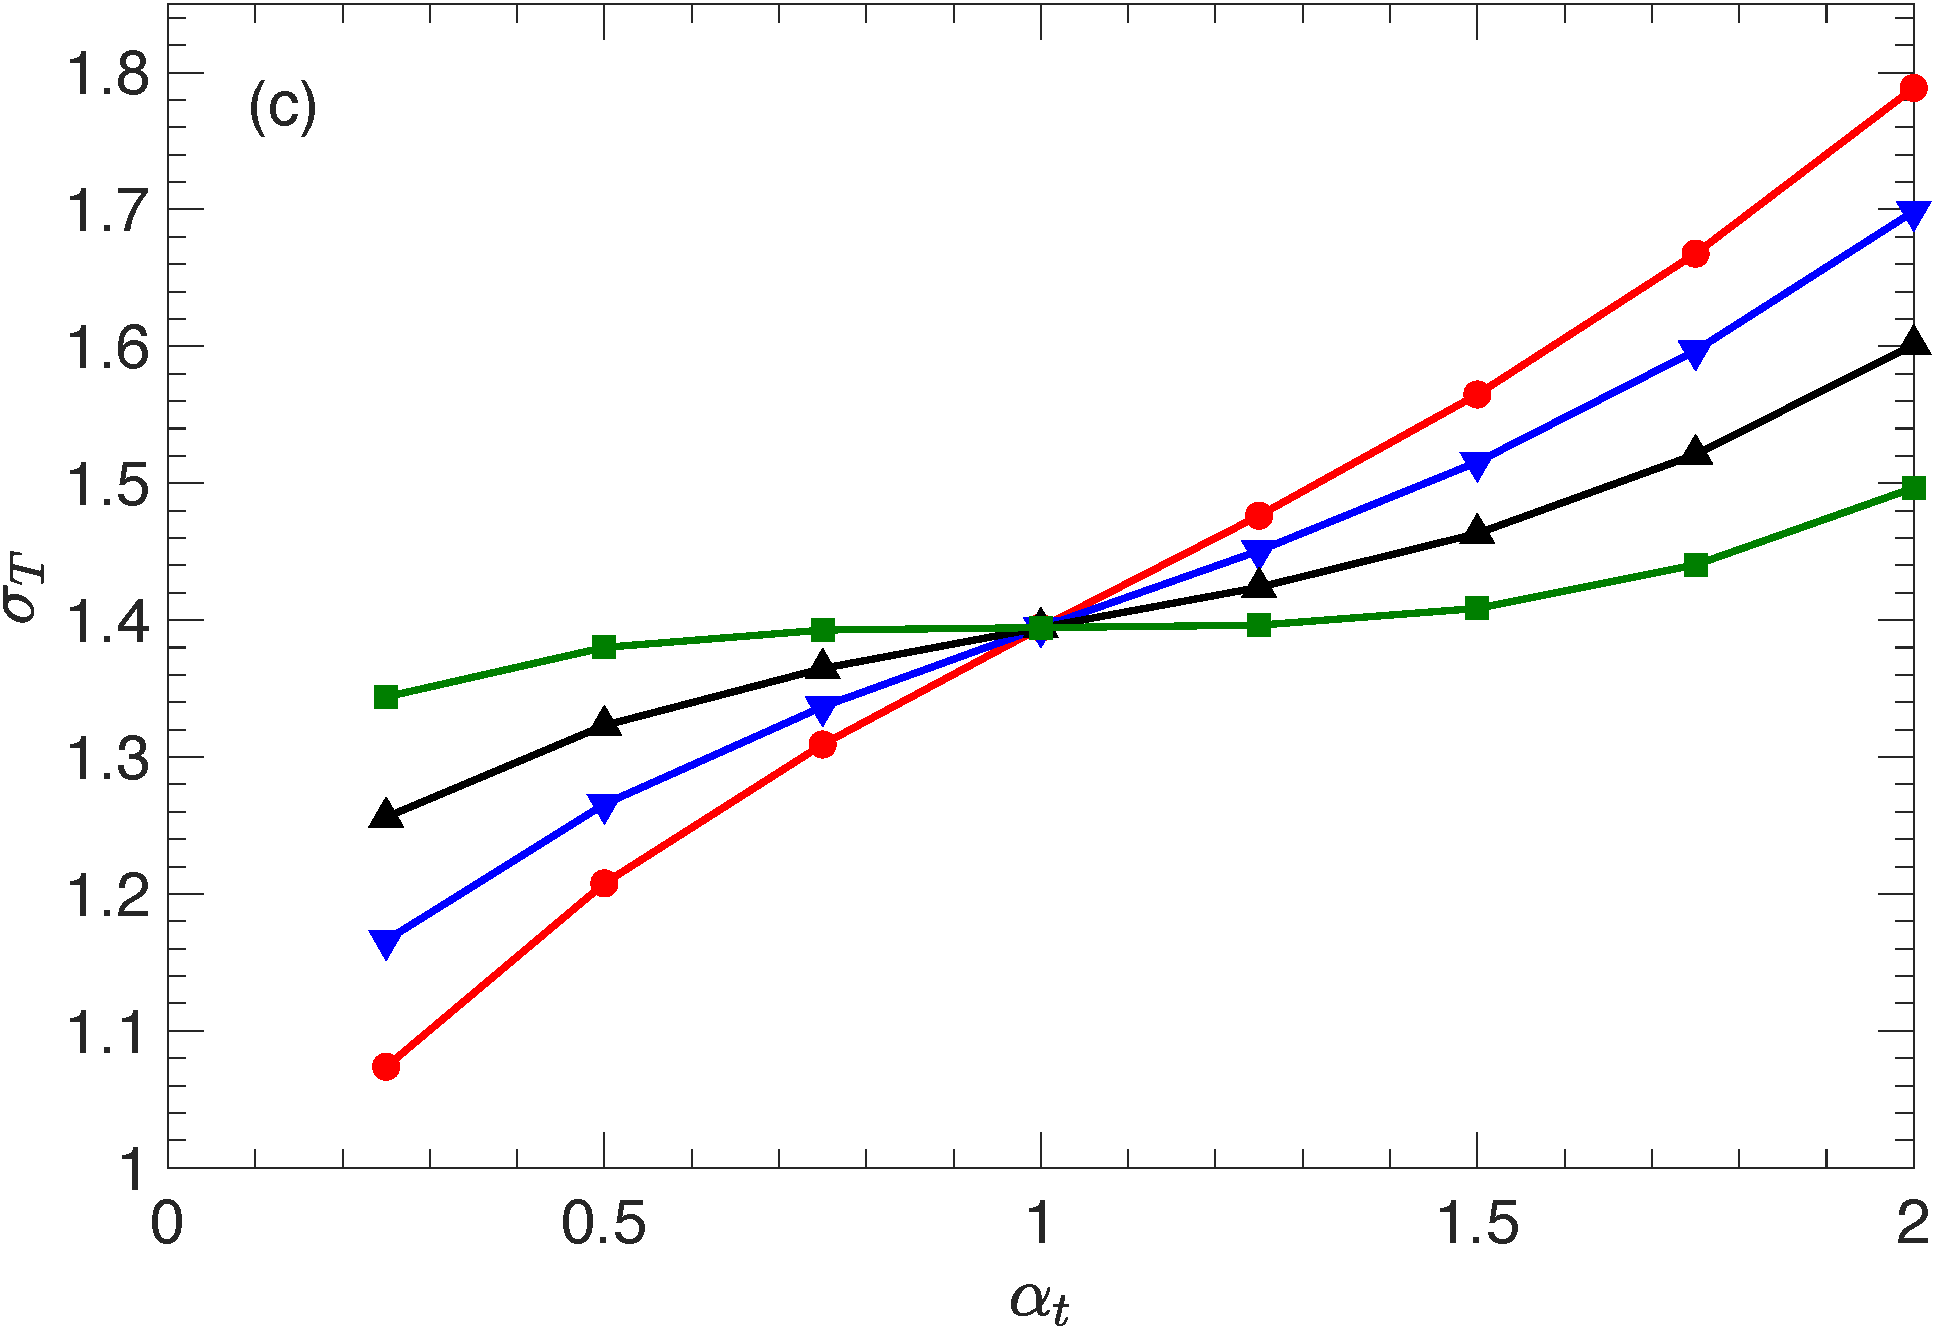
\includegraphics[width=0.45\textwidth]{SlipJump/IMG/TSC_vs_TMAC_Omega1p5}
	\caption{
		TSCs obtained from LBE for (a) HS, (b) Maxwellian, and (c) VHS ($\omega=1.5$) molecules, when the CLL BC is used. 
	}
\label{fig:TSC_Bound}
\end{figure}

Table~\ref{table_CL} and Fig.~\ref{fig:TSC_Bound} summarize the TSC computed from the LBE for HS, Maxwellian, and VHS ($\omega=1.5$) molecules with the Cercignani-Lampis  BC . When $\alpha_t$ and $\alpha_n$ are fixed, the TSC increases with the viscosity index. For example, when the HS and VHS with $\omega=1.5$ are considered, the maximum relative difference reaches $58\%$ when $\alpha_t=2$ and $\alpha_n=1$. When the viscosity index is fixed, however, the variation of TSC with respect to the effective TMAC $\alpha_t$ and EAC $\alpha_n$ is complicated. We first consider the case when the value of $\alpha_t$ and the intermolecular potential are fixed. From Table~\ref{table_CL} we see that, when $\alpha_t<1$, the TSC increases with $\alpha_n$, where the maximum increment is less than $20\%$ when $\alpha_n$ varies from 0.25 to 1. Furthermore, this kind of variation reduces when $\alpha_t$ approaches 1; when $\alpha_t=1$, the Cercignani-Lampis  BC  is reduced to the fully diffuse one in this problem, and the TSC does not vary with $\alpha_n$; when $\alpha_t>1$, the variation of TSC on $\alpha_n$ reverses when compared to that of $\alpha_t<1$.
We then fix the value of $\alpha_n$ and the intermolecular potential to see how $\alpha_t$ affects the TSC.  Unlike the diffuse-specular BC where the TSC is nearly a linear function of TMAC, here the change of TSC with respect to $\alpha_t$ is nonlinear. Also, it is observed that the smaller the value of $\alpha_n$, the strong the variation in TSC with $\alpha_t$. 
%This is clearly seen for HS and VHS molecules whose viscosity indexes deviate from 1. 
For instance, when $\omega=0.5$ and $\alpha_n=0.75$, the TSC first decreases to a minimum value at $\alpha_t\approx 0.5$, then increases to a maximum value at $\alpha_t\approx 1.5$. This is not observed in the work~\cite{Sharipov2003CL}, where the Shakhov  model~\cite{Shakhov_S} is employed and the TSC always increases with $\alpha_t$ when $\alpha_n$ is fixed. 



\subsection{Knudsen layer function}
\index{Knudsen layer function!thermal transpiration}
\begin{figure}[t]
	\centering
	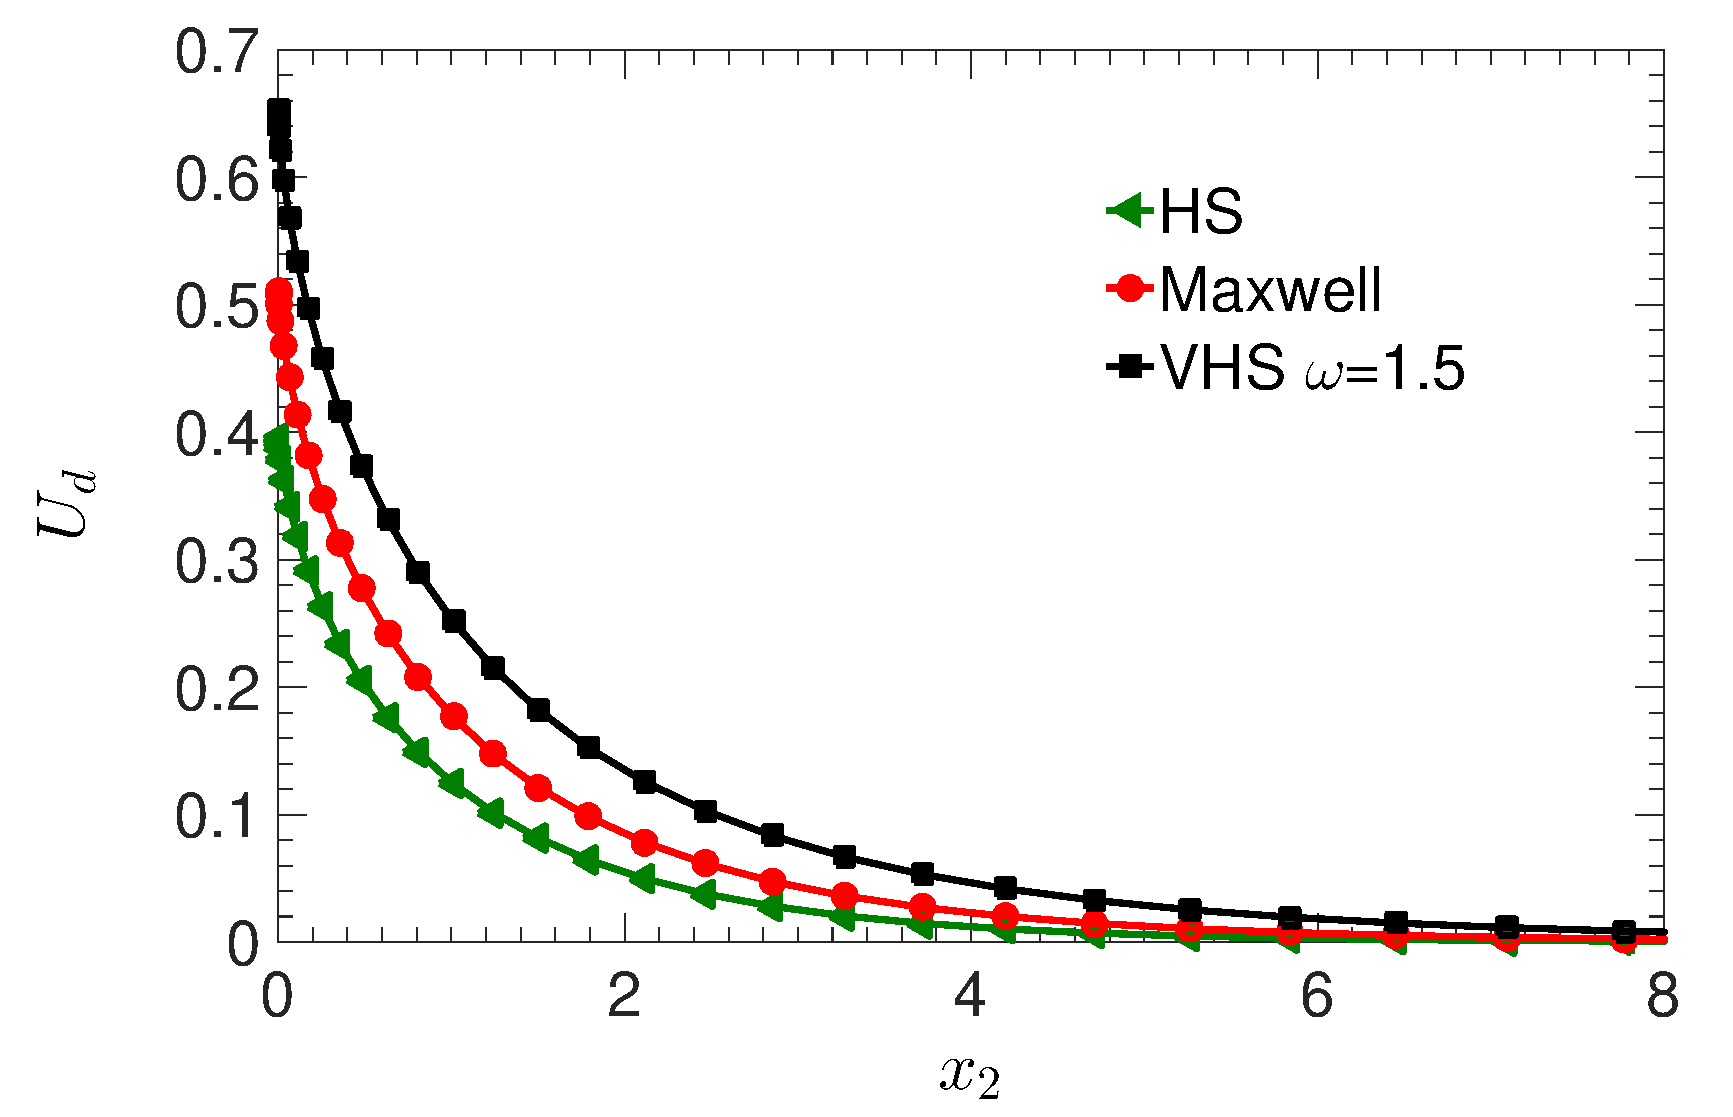
\includegraphics[scale=0.3]{SlipJump/IMG/Knudsenlayer}
	\caption{\label{fig:Ud_potential}KLFs obtained from the LBE for HS, Maxwellian, and VHS ($\omega=1.5$) molecules, when the diffuse BC is applied.  }
\end{figure}

The influence of intermolecular potential on the KLF has been rarely studied, even for monatomic gases, due to the complexity of the Boltzmann collision operator and the lack of efficient numerical methods to simulate the near-continuum flow. Fortunately, these computational difficulties can be tackled by the FSM and GSIS developed in previous chapters. 


Figure~\ref{fig:Ud_potential} shows the KLF obtained from the LBE for HS, Maxwellian, and VHS ($\omega=1.5$) molecules, when the diffuse BC is applied. Obviously, the KLF is strongly affected by the intermolecular potential, i.e. its value increases with the viscosity index $\omega$. For example, the value of the KLF at solid surface for VHS molecules with $\omega=1.5$ is larger than that of the HS molecules by approximately $60\%$. 


\begin{figure}[t]
	\centering
	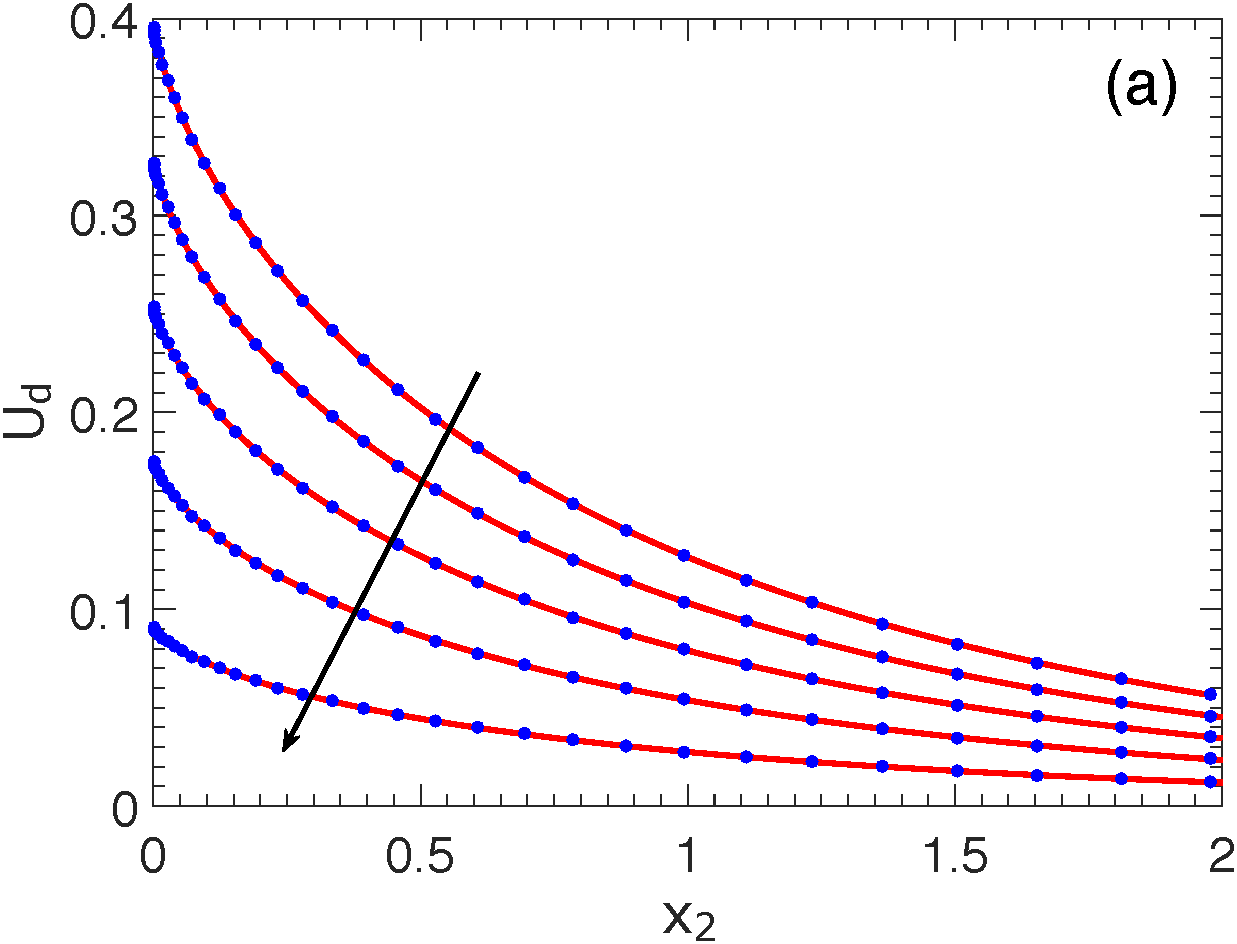
\includegraphics[scale=0.32]{SlipJump/IMG/KLF_am}
	\hskip 0.5cm
	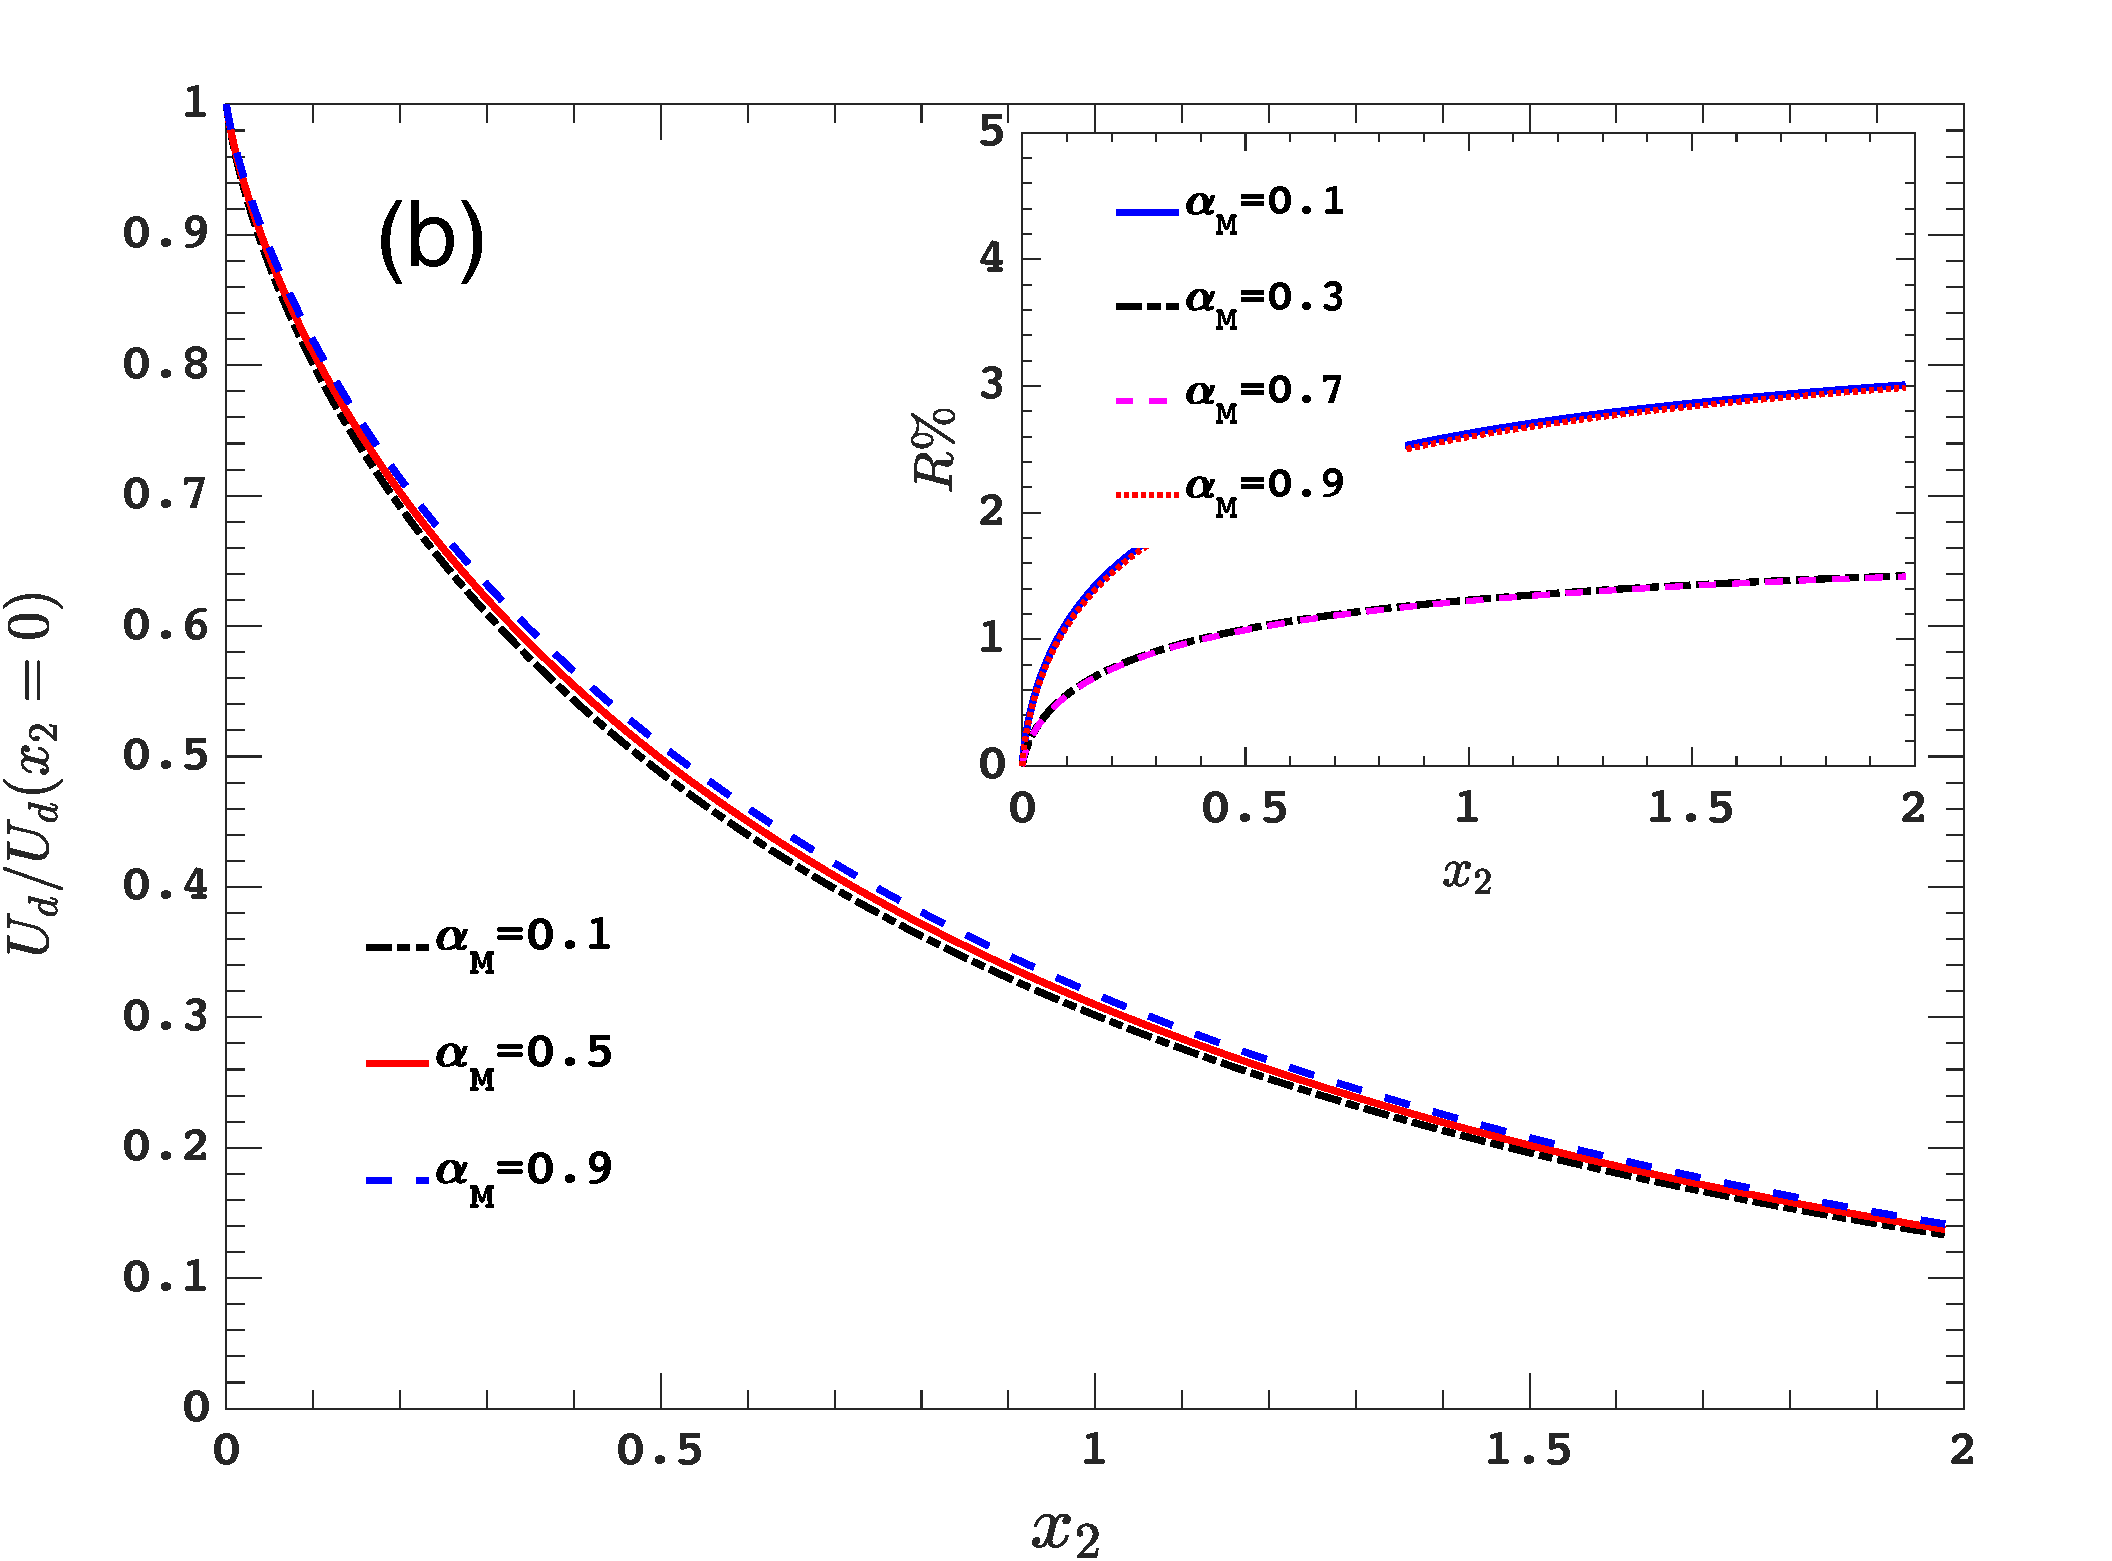
\includegraphics[scale=0.2]{SlipJump/IMG/KLF_similarity}
	\caption{
		(a) KLFs for HS molecules with the diffuse-specular BC. Along the arrow, the TMAC is $\alpha_M=1.0, 0.8, 0.6, 0.4$, and 0.2, respectively. Solid lines: LBE results; dots: fitting results by Eq.~\eqref{eq:vel_fit}.   $(b)$ The rescaled KLF $u_d(x_2)/u_d(0)$, when the HS molecules and diffuse-specular BC are used. For clarity, results at other values of $\alpha_M$ are not shown. Inset: the relative difference of the rescaled KLF for various $\alpha_M$ when compared to that of $\alpha_M=0.5$. }\label{fig:KLF_sim}
\end{figure}

Figure~\ref{fig:KLF_sim}$(a)$ further depicts the KLF when the specular-diffuse BC is used, from the case of $\alpha_M=0.2$  where the specular reflection is strong. It is noticed that the KLF decreases with the TMAC; this is in sharp contrast to the KLF in Kramer's problem where its value increases when the TMAC decreases~\citep{SU2019573}. However, both the thermal transpiration and Couette flow possess the singularity of velocity gradient at the planar surface. That is, $du_d/dx_2$ varies as $x_2\ln{}x_2$ in the vicinity of the wall, and such a gradient divergence is general in RGD~\citep{takata2013singular}. This conclusion holds also in the Couette flow described by the BGK kinetic model~\citep{Jiang2016JCP}, where the asymptotic analysis demonstrates that the KLF near the boundary can be described by Eq.~\eqref{eq:vel_fit}.
Interestingly, through numerical simulation and fitting, we find that the KLF in thermal transpiration can also be perfectly fitted by the same function,  where the fitting coefficients are listed in  Ref.~\cite{Wang2020PoF}.


Under the diffuse-specular BC, the similarity in KLF is found, that is, when the KLFs are rescaled by their values on the solid surface, they almost overlap with each other [Fig.~\ref{fig:KLF_sim}$(b)$]. This happens not only for HS molecules, but also for other intermolecular potentials. 




The KLFs are also obtained from the LBE with the Cercignani-Lampis BC. When $\alpha_t$ and $\alpha_n$ are fixed, the KLF increases with the viscosity index. However, unlike the diffuse-specular BC, the KLF only exhibits weak similarities when either $\alpha_t$ or $\alpha_n$ is fixed.
%. Therefore, there profiles are only shown in supplementary data. {\color{red} please provide supplementary files. (NEED to do!) }


%\subsection{MFR: the second-order contribution from KLF\label{mfr_2ndorder}}
%
%
%It is very hard to measure the TSC and KLF directly; instead, the mass flow rate and TPD exponent are measured. Since the TPD exponent is strongly related to the mass flow rate, here we quantify the influence of intermolecular potential and gas-surface BC on the mass flow rate in the near-continuum and early transition flow regimes.
%
%\begin{table}[t]
%	\centering
%	\caption{\label{table_CL_Ud}The area of Knudsen layer function $Q_d$ for various intermolecular potentials when the Cercignani-Lampis  BC  is used. Results of $\alpha_t=1$ are not shown as $Q_d$ are the same as those from the diffuse BCs in Table~\ref{table_rescale_coe}, irrespective of the value of $\alpha_n$.}
%		\begin{tabular}{lccccr}
%			\hline
%			$\alpha_t$  & $\omega$
%			&  $\alpha_n=0.25$ & $ \alpha_n=0.5$  &    $\alpha_n=0.75$ &    $\alpha_n= 1$\\
%			%%  \rowcolor[gray]{.9}
%			$0.25$
%			& 0.5   & 0.3730    & 0.4926  & 0.6081 & 0.7201  \\
%			&1.0    & 0.5648    & 0.7140   &  0.8580 & 0.9973  \\
%			&1.5    & 0.8827  & 1.0901   & 1.2869 &  1.4729  \\
%			%   \rowcolor[gray]{.9}
%			$0.5$
%			& 0.5   & 0.5219   & 0.5987   & 0.6738 & 0.7472  \\
%			&1.0    & 0.7967   & 0.8922    & 0.9855 & 1.0767 \\
%			&1.5    & 1.2432   & 1.3741   & 1.4995 &  1.6192  \\
%			
%			$0.75$
%			& 0.5   & 0.6462   & 0.6836   & 0.7204  & 0.7568 \\
%			&1.0    & 0.9675   & 1.0138    & 1.0595 & 1.1047 \\
%			&1.5    & 1.4883   & 1.5511   & 1.6119 & 1.6705  \\
%			
%			%   \rowcolor[gray]{.9}
%			$1.25$
%			& 0.5   & 0.8672   & 0.8314   & 0.7955 &  0.7595 \\
%			&1.0    & 1.2454   & 1.2014     & 1.1571 & 1.1125\\
%			&1.5    & 1.8609   & 1.8013   &1.7427 &  1.6849  \\
%			
%			%   \rowcolor[gray]{.9}
%			$1.5$
%			& 0.5   & 0.9813   & 0.9114   & 0.8405 & 0.7688  \\
%			&1.0    & 1.4008   & 1.3149  & 1.2280 & 1.1396  \\
%			&1.5    & 2.0828   & 1.9655   & 1.8497 & 1.7345  \\
%			
%			%   \rowcolor[gray]{.9}
%			$1.75$
%			& 0.5   & 1.1063   & 1.0041   & 0.8997   & 0.7930\\
%			&1.0    & 1.5928   & 1.4678    & 1.3405 & 1.2100  \\
%			&1.5    & 2.3807   & 2.2069   & 2.0352   &  1.8631  \\
%			
%			$2$
%			& 0.5   & 1.2439   & 1.1121   &0.9762 & 0.8361\\
%			&1.0    & 1.8312   & 1.6699    &1.5052 & 1.3351   \\
%			&1.5    & 2.7784   & 2.5475   &2.3196 &  2.0905\\
%			\hline	
%		\end{tabular}
%\end{table}
%

%\begin{figure}
%	\centering
%	\includegraphics[scale=0.3]{MFR2.pdf}
%	\caption{\label{fig:MFR}The normalized mass flow rate $Q$ vs $1/\delta_{rp}$ when the diffuse BC is used. Squares, dash-dot line, and dot line represent the results of HS molecules calculated from the LBE,  Eq.~\eqref{eq:MFR}, and the analytical solution with the first-order slip BC (i.e. $Q_1=\sigma_T/2\delta_{rp}$), respectively. Triangles, solid line, and dash line are the corresponding results for Maxwellian molecules.}
%\end{figure}
%
%
%The comparison of mass flow rate computed from the LBE and Eq.~\eqref{eq:MFR} for HS and Maxwellian molecules are shown in Fig.~\ref{fig:MFR}. Note that the mass flow rate $Q_1=\sigma_T/2\delta_{rp}$ obtained from the analytical solution with the first-order thermal slip BC is also plotted in the figure. 
%It is clear that, the mass flow rate computed from $Q_1$ is only in good agreement with the LBE result at a large value of $\delta_{rp}_{rp}\ge100$, while that from Eq.~\eqref{eq:MFR} agree well with the LBE results of $Q$ in the interval of $\delta_{rp}_{rp}\ge5$. For example, in the case of $\delta_{rp}_{rp}=5$, when compared with results of LBE for HS molecules, the relative error in the mass flow rate for Eq.~\eqref{eq:MFR} is smaller than $5\%$, while it is larger than $40\%$ for $Q_1$. The reason that Eq.~\eqref{eq:MFR} does not work well when $\delta_{rp}_{rp}<5$ is that the KLFs at two solid surfaces start to overlap and higher-order corrections are needed. %We also note that the discrepancy is even more pronounced for the Maxwellian molecules.


%Although the TSC increases with the viscosity index when other parameters are fixed, the KLF and hence $Q_d$ also increase with the viscosity index. Therefore, from~\eqref{eq:MFR} it may concluded that at large values of the Knudsen number, gas with smaller value of viscosity index may have a larger mass flow rate. This is observed in Fig.~\ref{fig:largeKn} below when $\text{Kn}>0.6$.


\subsection{Molecular gases}\label{sec:results2}
\index{molecular gas}
\index{translational Eucken factor}

So far no work has been devoted to finding the TSC and KLF of molecular gases based on the Boltzmann equation, although they can be roughly extracted from the numerical data given by Loyalka \textit{et al.}~\cite{loyalka1982thermal} and Lo \& Loyalka~\cite{lo1989flow}, where the thermal transpiration of molecular gases along planar channels and circular tubes were calculated based on the Hanson \& Morse kinetic model~\cite{Hanson1967PoF}. However, this model is proposed only for Maxwellian molecules, so the influence of intermolecular potential cannot be captured. 

\index{kinetic model !Wu}

Based on the numerical solution of the Wu model~\cite{LeiJFM2015}, we find TSC in the diffuse-specular BC can be fitted by 
\begin{equation}\label{eq:tsc_tmac_ftr}
\sigma_T=f_{tr}\left(C_1 \alpha_M+0.31\right),
\end{equation}
where the fitting coefficients are $C_1=0.095, 0.125$, and 0.165,  for $\omega=0.5$, 0.75, and 1, respectively. % $C_2$ at various intermolecular potentials are listed in Table~\ref{table:vsc_ftr_tmac}. 
For the Cercignani-Lampis  BC, when $\alpha_t$ does not deviate too much from 1, say, when $|\alpha_t-1|<0.3$, the TSC $\sigma_T(\alpha_n,\alpha_t)$ can be expressed as
\begin{equation}\label{CLL_simi}
\sigma_T(\alpha_n,\alpha_t)=\frac{2}{5}f_{tr}\sigma_T^m(\alpha_n,\alpha_t),
\end{equation}
where $\sigma_T^m(\alpha_n,\alpha_t)$ is the TSC for monatomic gas, see typical values in Table~\ref{table_CL}. The relative error between the Wu model and Eq.~\eqref{CLL_simi} increases when $\alpha_t$ further deviates away from one and $f_{tr}$ deviates away from 2.5, e.g. to 7\%  when $\alpha_t=0.2$ and $f_{tr}=0.5$.

%We notice that the relative error between the fitting and numerical solutions of the Wu model is within $2\%$, when $0.2\le\alpha_M\le1$ and $0.3\le{}f_{tr}\le2.5$. 
%
%\begin{table}[t]
%	\centering
%	\caption{\label{table:vsc_ftr_tmac} When the diffuse-specular BC is applied, the TSC of molecular gases can be fitted according to Eq.~\eqref{eq:tsc_tmac_ftr}.}
%		\begin{tabular}{ccc}
%			\hline
%			$\omega$  &  $C_1$ & $C_2$   \\
%			0.5       &0.095  & 0.310     \\
%			0.75      &0.125  & 0.309    \\
%			1.0       &0.165  &0.305   \\
%			1.25      &0.202  &0.304   \\
%			\hline
%		\end{tabular}
%\end{table}





%\subsection{Knudsen layer function}


\begin{figure}[t]
	\centering
	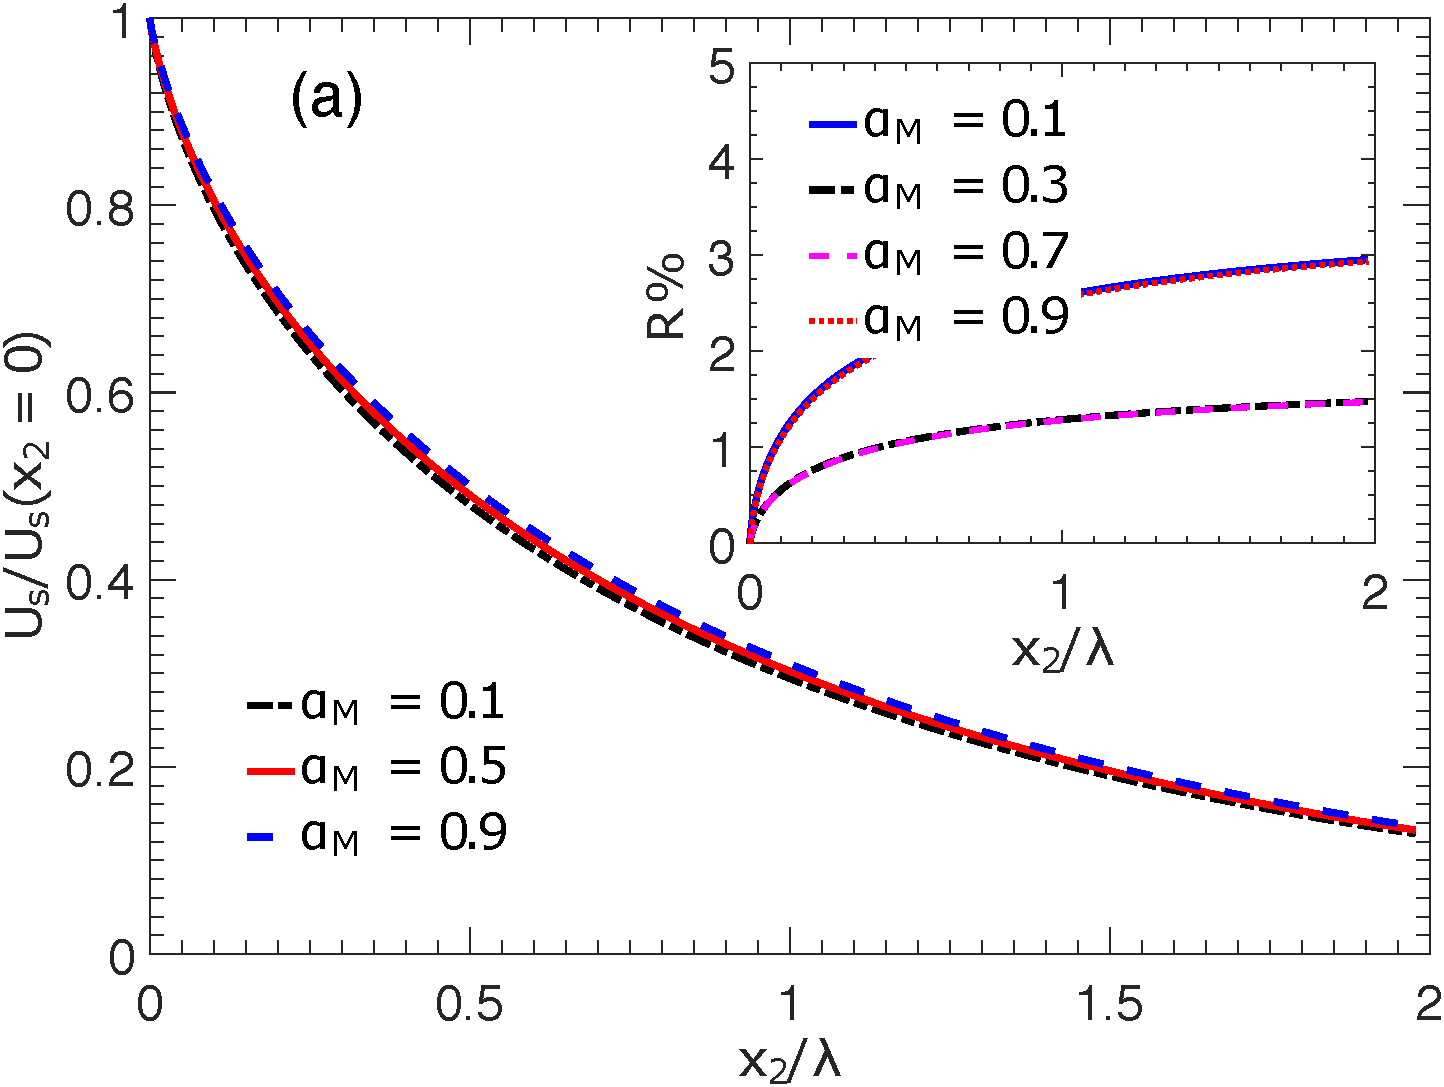
\includegraphics[scale=0.25]{SlipJump/IMG/KLF_d2Z5.pdf}
	\hskip 20pt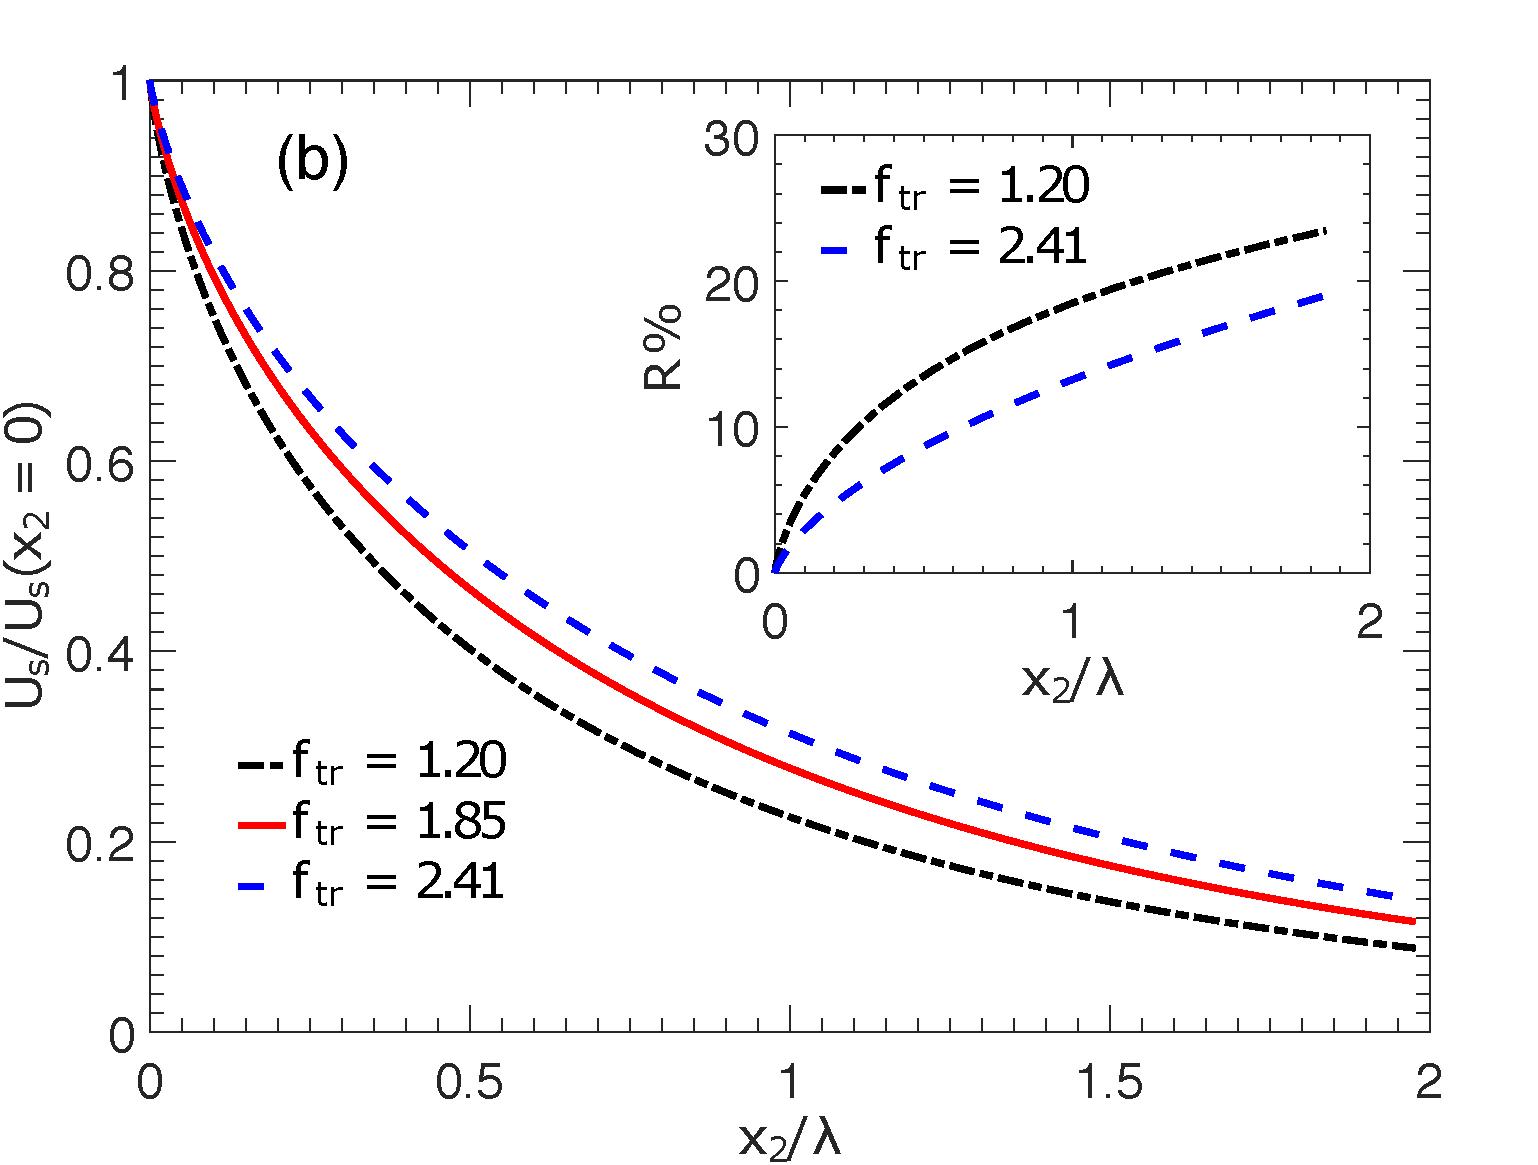
\includegraphics[scale=0.25]{SlipJump/IMG/Ud_ftr_d2.pdf}
	\caption{\label{fig:Ud_rotation}The rescaled KLF $u_d(x_2)/u_d(0)$ obtained from the Wu model for the HS molecules, subject to the diffuse-specular BC. (a)  The diffuse-specular BC at different $\alpha_M$ is applied with $f_{tr}=2.37$. Inset: the relative difference of the rescaled KLF for various $\alpha_M$ when compared to that of $\alpha_M=0.5$. (b) The fully diffuse BC is applied with different $f_{tr}$. Inset: the relative difference of the rescaled KLF for various $f_{tr}$ when compared to that of $f_{tr}=1.85$.}
\end{figure}




Like the monatomic gas, the KLF of molecular gases holds similarity at different TMAC when the diffuse-specular BC is applied; this is demonstrated in Fig.~\ref{fig:Ud_rotation}(a), where the rescaled KLFs as well as their relative difference are presented.
It is clearly seen that the rescaled KFLs for $\alpha_M=0.1, 0.5$ and 0.9 almost overlap with each other,  and their maximum derivation from that of $\alpha_M=0.5$ is within $3\%$. Interestingly, although the TSC is proportional to the translational Eucken factor $f_{tr}$, the rescaled KLF does not preserve the similarity with respect to $f_{tr}$. As presented in Fig.~\ref{fig:Ud_rotation}(b), the rescaled KLF profiles for $f_{tr}=1.2, 1.85$ and 2.41 have large discrepancies. 






\subsection{Comparison with experiments\label{sec:results3}}


Experimental data on thermal transpiration of air and carbon dioxide in a circular tube are examined by the LBE calculations. From the discussions in previous sections we know that these data depend on the values of $f_{tr}$, $\omega$, and TMAC. The same problem has been investigated by Loyalka \textit{et al.}~\cite{loyalka1982thermal} based on the Hanson \& Morse model~\cite{Hanson1967PoF} that is derived from the Wang-Chang \& Uhlenbeck equation~\cite{WangCS} for Maxwellian molecules, but with the diffuse BC only. The methodology we will adopt has two major advantages. First, in the Wu model~\cite{LeiJFM2015} for molecular gases, the viscosity index can be properly chosen to reflect the intermolecular potential for each gas, which is not accessible in previous molecular gas models. Second, $f_{tr}$ is extracted from the experiments of Rayleigh-Brillouin scattering, where the gas-surface interaction is absent so that it is obtained accurately~\citep{Wu2020JFM}. Therefore, in the comparison between our LBE and experiential results, the gas-surface BC in thermal transpiration can be extracted with good accuracy.


In the experiment of thermal transpiration usually the TPD exponent $\gamma$ is measured. When the temperature ratio of two gas reservoirs connected by a long circular tube is small, the TPD exponent can be calculated as
\begin{equation}
\gamma=-\frac{Q_{T}}{Q_P},
\end{equation}
where $Q_{T}$ and $Q_P$ are the mass flow rates along the tube in thermal transpiration and Poiseuille flows, respectively. 


In the slip regime, with the aid of first-order slip BC, the dimensionless mass flow rate of the Poiseuille flow $Q_P$ in a circular tube is~\citep{sharipov2015rarefied}
\begin{equation}\label{Su_JCP_VSC}
Q_P=\frac{\delta_{rp}}{8}+\frac{\sigma_P}{2},
\end{equation}
where the VSC is set to $\sigma_P=1$, 1.2 and 1.46 for the cases of $\alpha_M=1$, 0.9 and 0.8, respectively, as the intermolecular potential has negligible effect on these values~\citep{SU2019573}. Note that Eq.~\eqref{Su_JCP_VSC} is accurate when $\delta_{rp}>10$. 


When $\delta_{rp}$ is large such that the two Knudsen layers do not overlap, from Eqs.~\eqref{NS_fit} and~\eqref{slip_coe} we find that the normalized mass flow rate $Q$ can be calculated exactly as
\begin{equation}\label{eq:MFR}
Q=\frac{\sigma_T}{2\delta_{rp}}-\frac{\pi}{4\delta_{rp}^2}Q_d,
\end{equation}
where 
\begin{equation}
Q_d=\int_0^\infty{}u_d(x_2)d x_2,
\end{equation}
is the mass flow rate correction due to defect velocity, whose values for typical values of viscosity index are listed in Ref.~\cite{Wang2020PoF} when the Cercignani-Lampis  BC  is used. It is seen from Eq.~\eqref{eq:MFR} that the KLF provides a correction of the mass flow rate up to the second-order of Knudsen number.


The analytical solution of TPD exponent in the slip regime can be written as
\begin{equation}\label{eq:analytical}
\gamma=\frac{4\sigma_T\delta_{rp}-2\pi Q_d}{\delta_{rp}^2(\delta_{rp}+4\sigma_P)}.
\end{equation}



In our LBE simulations, the viscosity index $\omega$ for each gas is set according to the gaseous property~\citep{Bird1994}. With the values of $Q_d$, $\sigma_T$, and $\sigma_P$ at a specific $\alpha_M$ obtained from previous sections, the analytical solution~\eqref{eq:analytical} for the TPD exponent can be determined, which will be used to extract the TMAC by comparing with the experimental data when $\delta_{rp}>3.5$.
 
%As a matter of fact, results in Fig.~\ref{fig:Air} show that when $\delta_{rp}\gtrsim 3.5$ ($\text{Kn}\lesssim 0.25$), the analytical solution~\eqref{eq:MFR}  at each value of TMAC agrees excellently well with the computational results from the LBE for air. 
Then we solve the Wu model towards smaller values of $\delta_{rp}<3.5$ to see whether our results still agree with experimental data or not.



\begin{figure}\centering
	{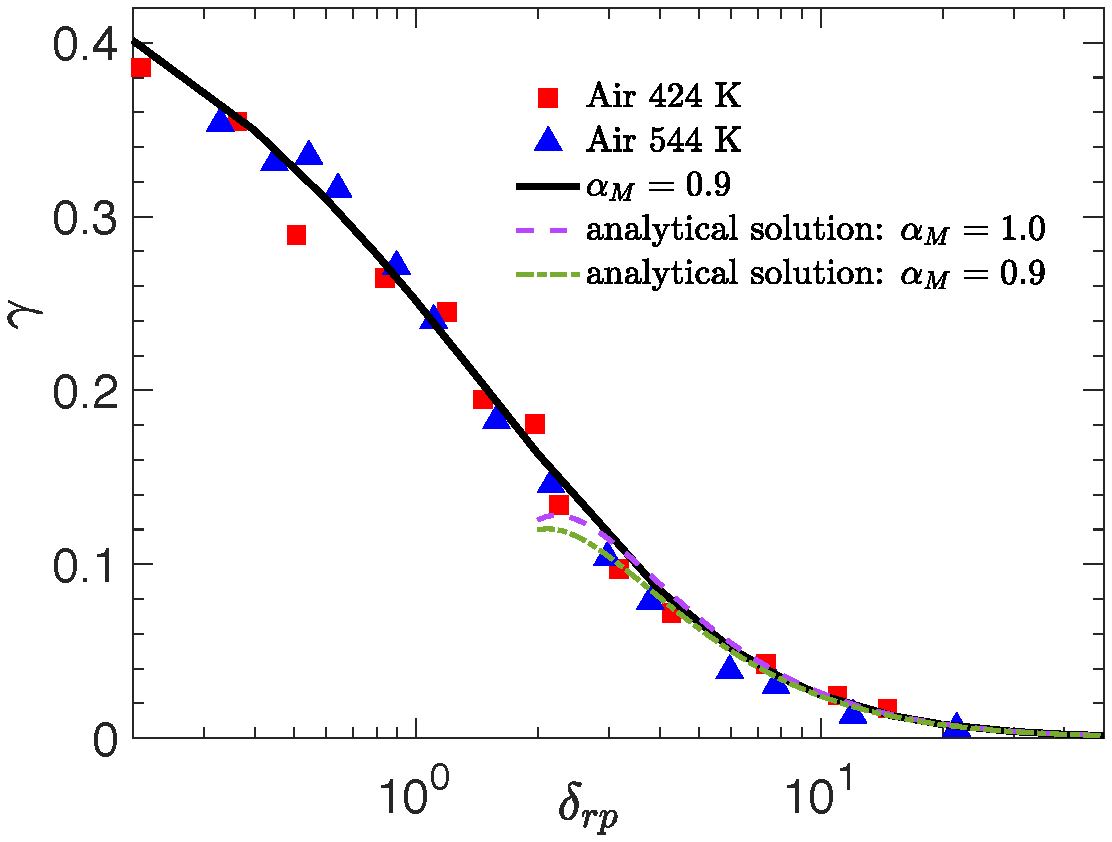
\includegraphics[scale=0.34]{SlipJump/IMG/Air_peng_new.pdf}}
	\hskip 0.5cm
	{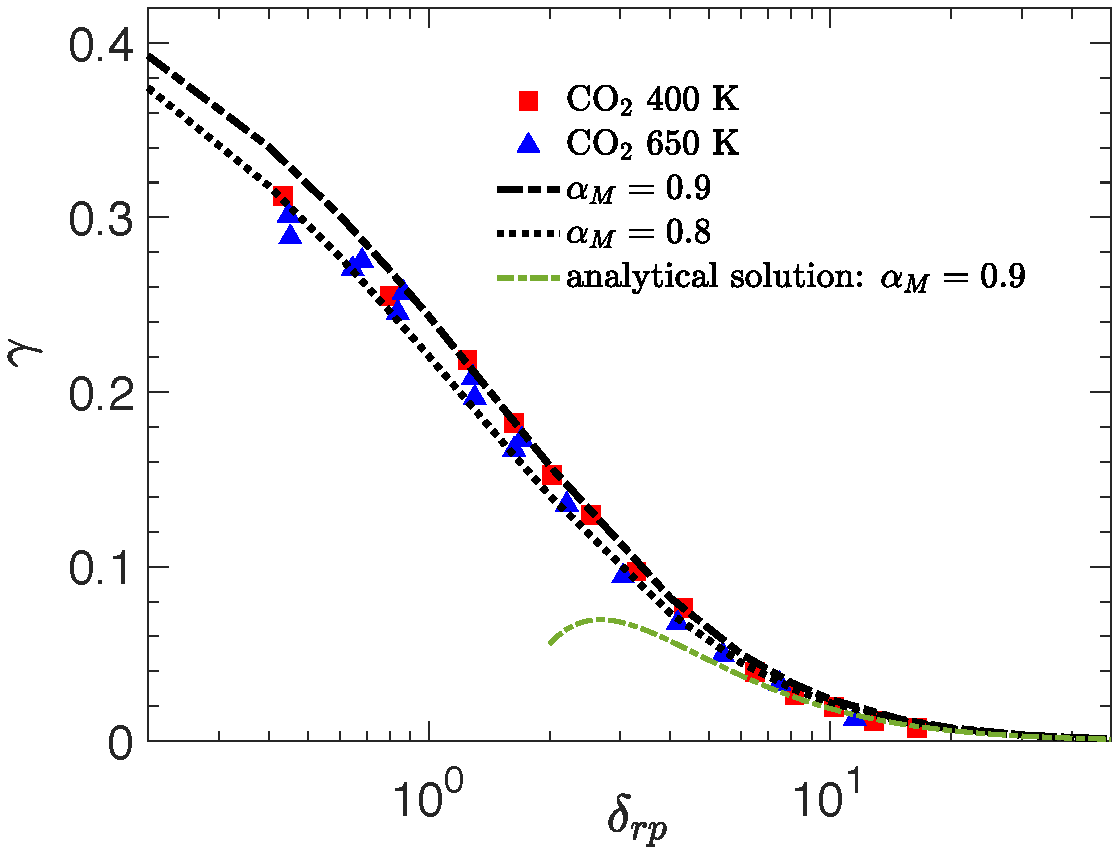
\includegraphics[scale=0.34]{SlipJump/IMG/CO2_peng_new.pdf}}
	\caption{\label{fig:Air}TPD exponent versus the rarefaction parameter $\delta_{rp}$, for air (left) and carbon dioxide (left) flows along a circular tube. Symbols: experimental data extracted from reference~\cite{arney1962addendum}. Black lines: numerical solutions of the Wu model~\cite{LeiJFM2015}.
		The analytical solution is given by Eq.~\eqref{eq:analytical}. 
	}
	
\end{figure}

\subsubsection{Air}

We first compare the calculated TPD exponent of thermal transpiration for air with the experimental data by Arney and Bailey~\cite{arney1962addendum} in Fig.~\ref{fig:Air}. Since air is mainly the mixture of nitrogen and oxygen, an effective viscosity index of $\omega=0.75$ is chosen to reproduce the proper intermolecular potential of the air molecules~\citep{Bird1994,SU2019573}. %The experimental data obtained by are used because separation of the components by thermal diffusion does not occur. 
The number of rotational degrees is $2$. The translational Eucken factor is $f_{tr}=2.4$ as extracted from the Rayleigh-Brillouin experiments of nitrogen~\citep{Wu2020JFM}. We first use the analytical expression~\eqref{eq:analytical} to obtain the TMAC by comparing with the experimental data at $\delta_{rp}>10$.  From the results in previous sections, the TSC can be extracted from the linear function 
\begin{equation}\label{eq:tsc_df}
\sigma_T=0.294\alpha_M+ 0.752,
\end{equation} 
and the mass flow rate correction $Q_d$ for air can be calculated from 
\begin{equation}\label{eq:air}
Q_d=4.182\left[1-\exp(-0.228 \alpha_M)\right].
\end{equation}
We find that when $\alpha_M$ varies from 0.8 to 1, the results in Eq.~\eqref{eq:analytical} can cover almost all the experimental data at temperature $T=424$K and $544$K. Then we solve the Wu model over a wide range of rarefaction parameter and find that the TMAC in the air experiments is more likely $0.9$, rather than $\alpha_M=1$ used in the reference~\cite{loyalka1982thermal}.



\subsubsection{Carbon dioxide}






The comparisons of TPD exponent for CO$_2$ between the measurements and solutions of the Wu model are shown in Fig.~\ref{fig:Air}, where the effective viscosity index is set to 0.93, while the translational Eucken factor is $f_{tr}=2.24$ as extracted from the Rayleigh-Brillouin experiments of carbon dioxide~\citep{Wu2020JFM}. The rotational degrees is still equal to 2, since the three atoms in a CO$_2$ molecule line up. We estimate the values of TSC and the mass flow correction $Q_d$ as
\begin{equation}
\begin{aligned}[b]
\sigma_T=&0.271\alpha_M+ 0.576,\\
Q_d=&4.726\left[1-\exp(-0.207 \alpha_M)\right].
\end{aligned}
\end{equation} 
%Clearly, the same as the case of air, analytical solutions of~\eqref{eq:MFR} shown in Fig.~\ref{fig:CO2} for $\delta_{rp} \gtrsim 3.5$ are in excellent agreement with the LBE numerical results.


We can also see that, when $\delta_{rp}>1$ the experimental data at $T=400$K can be well reproduced by the Wu model when $\alpha_M=0.9$, while the data at a higher temperature of $T=650$ are more close to solutions of the Wu model  when $\alpha_M=0.8$. Note that the value of $\gamma$ at $\delta_{rp} \approx 0.45$ is even below the profile of $\alpha_M=0.8$, which may be attributed to the inaccurate experimental measurement at low gas pressures. Nevertheless, all experimental data almost fall between the profiles of $\alpha_M=0.8$ and 0.9, which suggest that the TMAC in the CO$_2$ experiment is more likely $\alpha_M=0.85\pm 0.05$. 


\section{Temperature jump}
\index{temperature jump coefficient}



The temperature jump coefficient is calculated from the linear fitting of the temperature profile, named $\tau_{NS}$, in the bulk region ($x_1\in[0.3,0.7]$), according to its definition~\eqref{Tjump} as
\begin{equation}
\zeta_T=-\frac{A+1}{2kA},
\end{equation}
where $A$ is the slope coefficient in the linear fitting
\begin{equation}
\tau_{NS}\left(x_1\right)=A\left(x_1-\frac{1}{2}\right)\Delta\tau,
\end{equation}
with $\Delta\tau=\Delta T/T_0$ the perturbation of wall temperature. The Knudsen lay function, i.e., defective temperature $\Theta$, is obtained by comparing the kinetic solution and the linear fitting within Knudsen layer
\begin{equation}
\Theta\left(x_1\right)=\frac{1}{Ak\Delta\tau}\left(\tau_{NS}-\tau\right).
\end{equation}
We separately consider the translational and rotational temperatures, as the KLFs are different. However,  the jump coefficients are the same. 


In this section, we use the values of $Z$ and $\bm{A}$ extracted from the direct simulation Monte Carlo (DSMC) method~\cite{Wu2020JFM,Li2021JFM}:  $Z=2.667$, $A_{tt}=0.786$, $A_{tr}=-0.201$, $A_{rt}=-0.059$, and $A_{rr}=0.842$, thus $f_{tr}=2.365$ and $f_{rot}=1.435$. %Note that these values are chosen to match the experimental thermal conductivity, or equivalently $f_{u}=1.993$ of nitrogen at $T_0=300$ K, therefore the given value of $Z$ may not lead to the correct bulk viscosity. The DSMC neither has mechanism to separately alert the components of thermal conductivity since all the $A_{ij}$ depend on the value of $Z$.

\subsubsection{Influence of intermolecular potential}\label{sec:elastic}

The translational and rotational Knudsen layer functions are plotted in Fig.~\ref{fig:KLF_w}. With the given $Z$ and $\bm{A}$, the rotational Knudsen layer functions are larger than the translational ones. When the viscosity index $\omega$ increases from 0.5 to 1, the jump coefficients slightly increase with magnitudes no larger than 3\%. The Knudsen layer functions also become larger, and maximum increments, occurring in the vicinity of wall, are about 0.115 and 0.048 for the translational and rotational ones, respectively.

Therefore, like monatomic gases, the temperature jump in molecular gases are not sensitive to the elastic collision rate. In the following sections, we will use the Wu model, where the elastic collision is described by the Shakhov model. Since the translational and rotational jump coefficients have little difference, we will not particularly distinguish the translational or rotational one when demonstrate the results.



\begin{figure}[t]
	\centering
	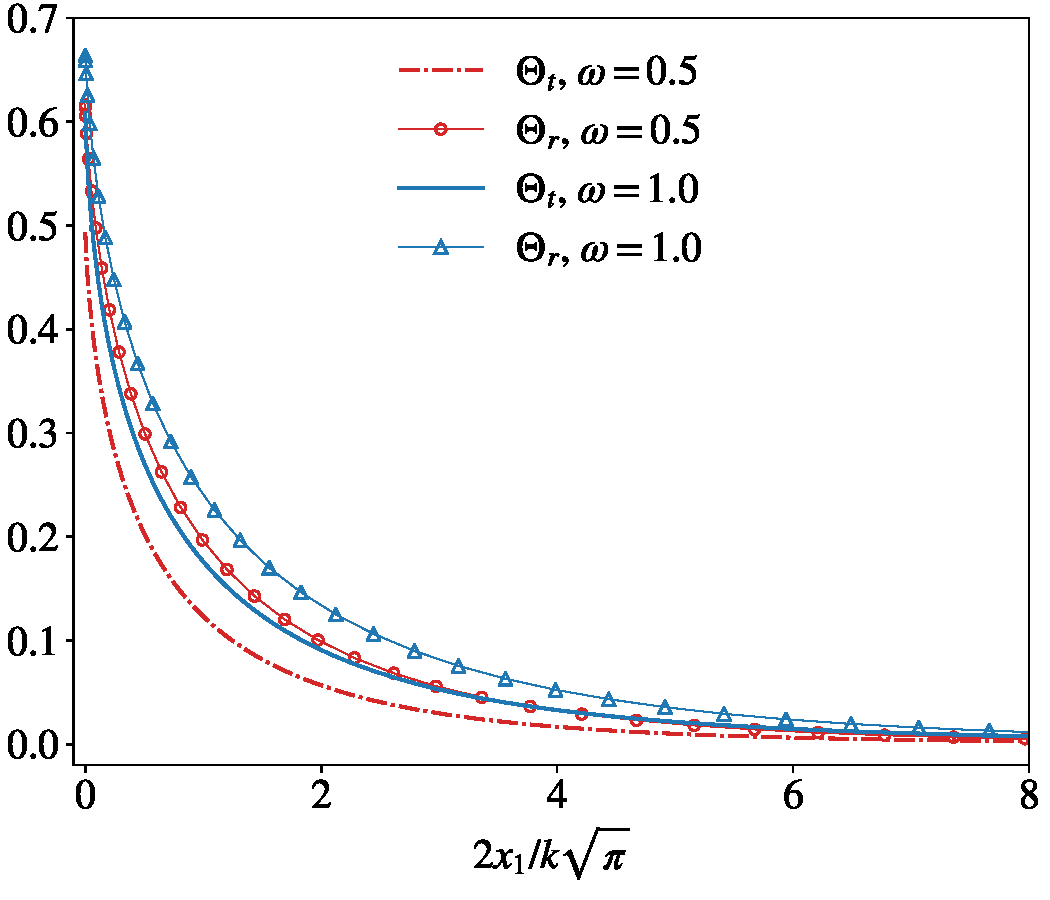
\includegraphics[width=0.5\columnwidth]{SlipJump/IMG/KLF_w}%
	\caption{The obtained Knudsen layer functions for the translational and the rotational temperatures when the modeling of elastic collision in the kinetic model~\eqref{Wu-linear-0} is replaced by the Boltzmann collision operator for a more realistic collision rate. The inverse law potential is consider with the viscosity index $\omega=0.5$ and $\omega=1.0$. }
	\label{fig:KLF_w}
\end{figure}


\index{Knudsen layer function!Fourier}

\subsubsection{Influence of rotational collision number}

Now we investigate the influence of the temperature relaxation~\eqref{relx_t} by changing $Z$ and keeping $A_{ij}$. The temperature jump coefficients $\zeta_T$ obtained with $Z$ equal to 1.0, 2.667 and 5.0 are listed in Table~\ref{tab:TJC_Z}. It is shown that $\zeta_T$ slightly increase as $Z$ becomes larger. The obtained translational and rotational Knudsen layer functions are plotted in Fig.~\ref{fig:KLF_Z}; when $Z=1.0$, i.e., the occurring of inelastic collisions that exchange translational and rotational energies is frequent, $\Theta_t$ and $\Theta_r$ are close, while as $Z$ increases to 5.0, i.e., the probability for inelastic collisions becomes smaller, the discrepancy between $\Theta_t$ and $\Theta_r$ enlarges. However, the variation is not significant.



\begin{figure}[t]
	\centering
	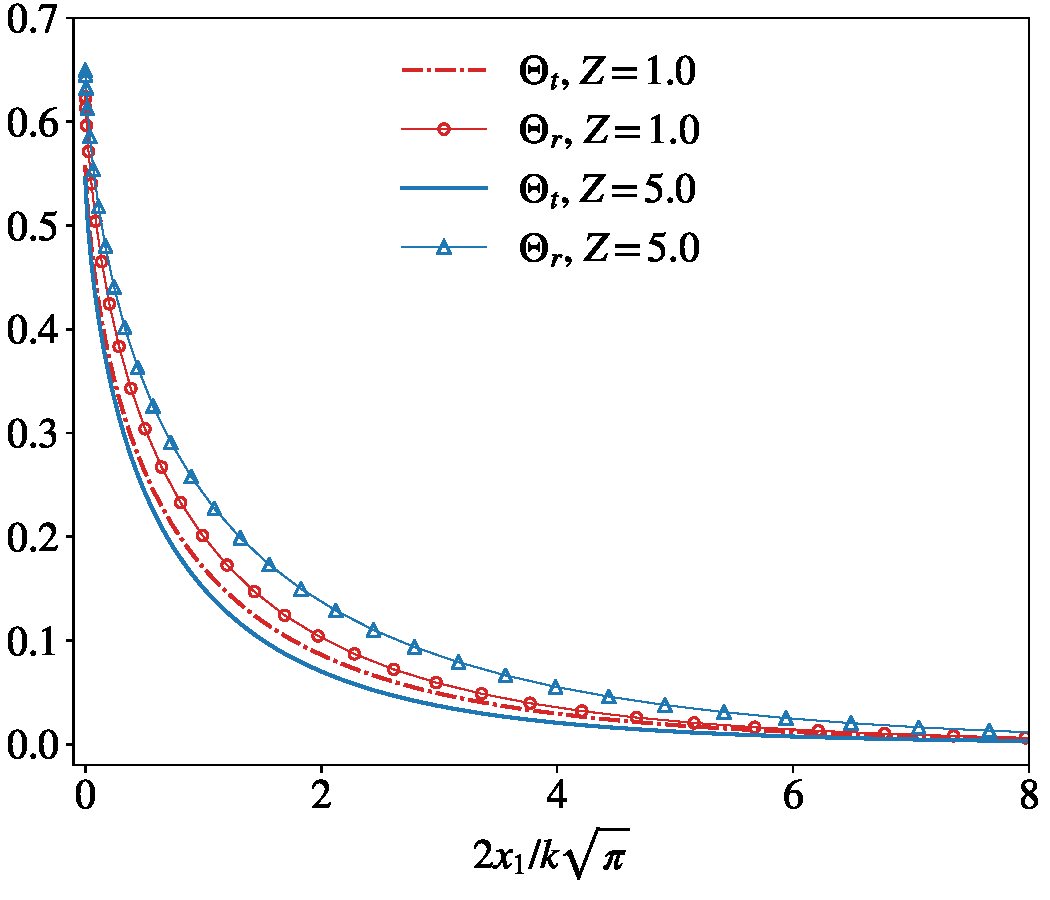
\includegraphics[width=0.5\columnwidth]{SlipJump/IMG/KLF_Z}%
	\caption{The Knudsen layer functions for the translational and the rotational temperatures with $Z=1.0$ and $Z=5.0$. }
	\label{fig:KLF_Z}
\end{figure}


\subsubsection{Influence of thermal relaxation}

Now we study the influence of thermal relaxations~\eqref{relx_q} by changing the relaxation rates and keeping $Z=2.667$. The thermal conductivity and its components will alert with $A_{ij}$, therefore in order to make duly comparisons, the total Eucken factor $f_{u}=1.993$ is kept as the experimental value for nitrogen at $T_0=300$ K. 

We first fix the cross terms $A_{tr}$ and $A_{rt}$ and alter $f_{tr}$ and $f_{rot}$ that are the percentages of translational and rotational contributions to the thermal conductivity. The diagonal terms $A_{tt}$ and $A_{rr}$ will correspondingly vary. Figure~\ref{fig:KLF_Ft}(a) displays the temperature jump coefficient against the translational Eucken factor, where the three lines relate to the three groups of cross terms: $A_{tr}=A_{rt}=0.0$ without cross exchange; $A_{tr}=-0.201$ and $A_{rt}=-0.059$ the ones extracted from the DSMC; $A_{tr}=-1.005$ and $A_{rt}-0.295$ that are 5 times larger, in magnitude, than those from the DSMC. It is found that the temperature jump coefficient first falls and then slightly rises as the translational Eucken factor increases (or the rotational Eucken factor decreases), and the minimum value that is about 1.715 appears when $f_{tr}$ is around $2.2\sim2.25$. The most significant variation of $\zeta_T$ when $f_{tr}$ changes from 1.5 to 2.5 occurs when the cross exchange in thermal relaxation is intensified ($A_{tr}=-1.005$ and $A_{rt}=-0.295$), where the minimum jump coefficient is about 86\% of the maximum one ($\zeta_T=1.9922$ at $f_{tr}=1.5$). The Knudsen layer functions are plotted in Fig.~\ref{fig:KLF_Ft}(b). We can find that, when $f_{tr}=1.5$ and $f_{rot}=2.733$, the translational Knudsen layer function $\Theta_t$ is larger than the rotational one $\Theta_r$, which means that $\Theta_t$ deviates more from the Navier-Stokes solution; while when $f_{tr}$ increases to 2.5 and $f_{rot}$ reduces, the situation reverses and now $\Theta_r$ is larger. When the two Knudsen layer functions meet in the middle at $f_{tr}=2.25$, the minimum temperature jump coefficient emerges. 



\begin{figure}[t]
	\centering
	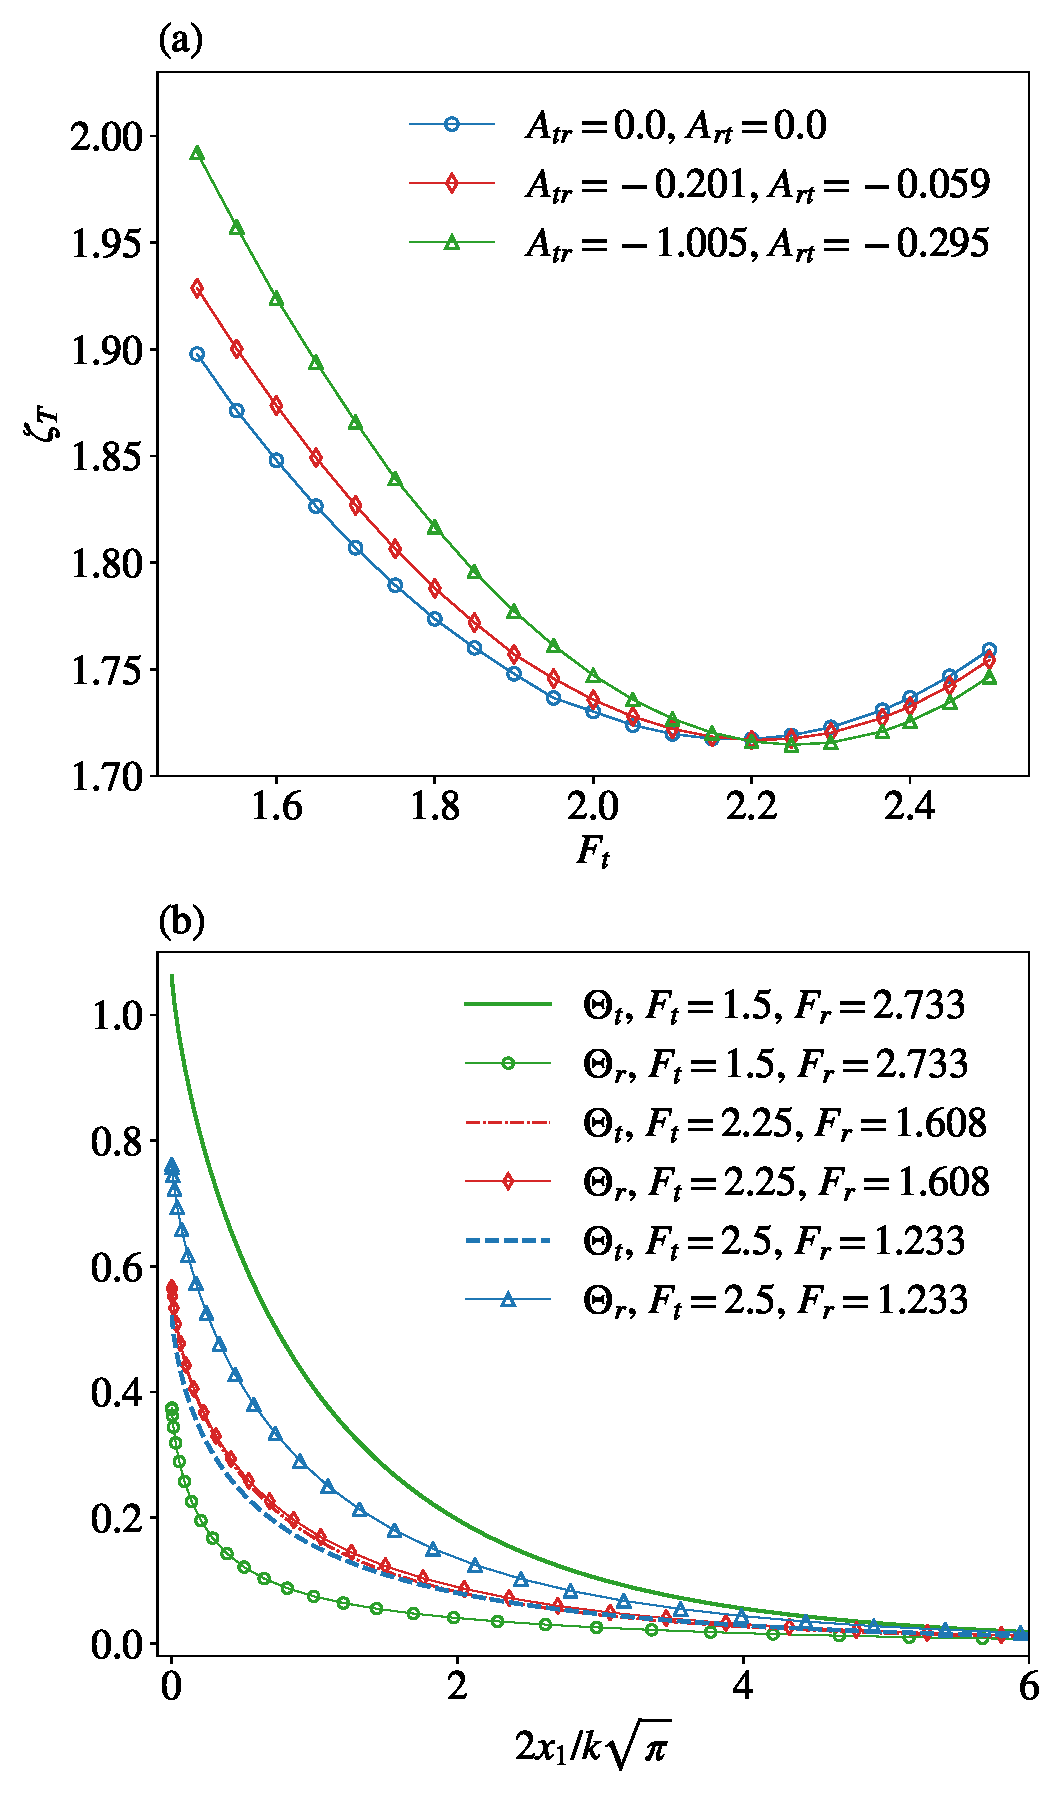
\includegraphics[width=0.4\columnwidth]{SlipJump/IMG/KLF_Ft}%
	\caption{(a) Temperature jump coefficient displaying the influence of the translational Eucken factor when $Z=2.667$, $f_{u}=1.993$, and the diagonal terms $A_{tt}$ and $A_{rr}$ altering. (b) Knudsen layer functions displaying the influence of the Eucken factors when $Z=2.667$, $f_{u}=1.993$, $A_{tr}=-1.005$ and $A_{rt}=-0.295$.}
	\label{fig:KLF_Ft}
\end{figure}

Then we fix $f_{tr}$ and $f_{rot}$, and check how the cross terms $A_{tr}$ and $A_{rt}$ affect the jump coefficient. Figure~\ref{fig:TJC_QtQr}(a) illustrates the obtained $\zeta_T$ when $A_{tr}$ varies and $A_{rt}$ is fixed as -0.059, where the two lines correspond to the results at $f_{tr}=1.5$ and 2.5, respectively. It is found that when $f_{tr}=1.5$, the translational part in the thermal conduction is relatively small, the jump coefficient increases as the magnitude of $A_tr$ becomes larger, that is the contribution to the relaxation of translational heat flux from the rotational one intensifies; while the jump coefficient decreases when $f_{tr}=2.5$, the translational part is relatively large. Figure~\ref{fig:TJC_QtQr}(b) shows the obtained $\zeta_T$ when $A_{tr}=-0.201$  and $A_{rt}$ varies. Now, as the magnitude of $A_rt$ becomes larger, that is the contribution to the relaxation of rotational heat flux from the translational one intensifies, the jump coefficient decreases at $f_{tr}=1.5$; while the jump coefficient increases at $f_{tr}=2.5$.

\begin{figure}[t]
	\centering
	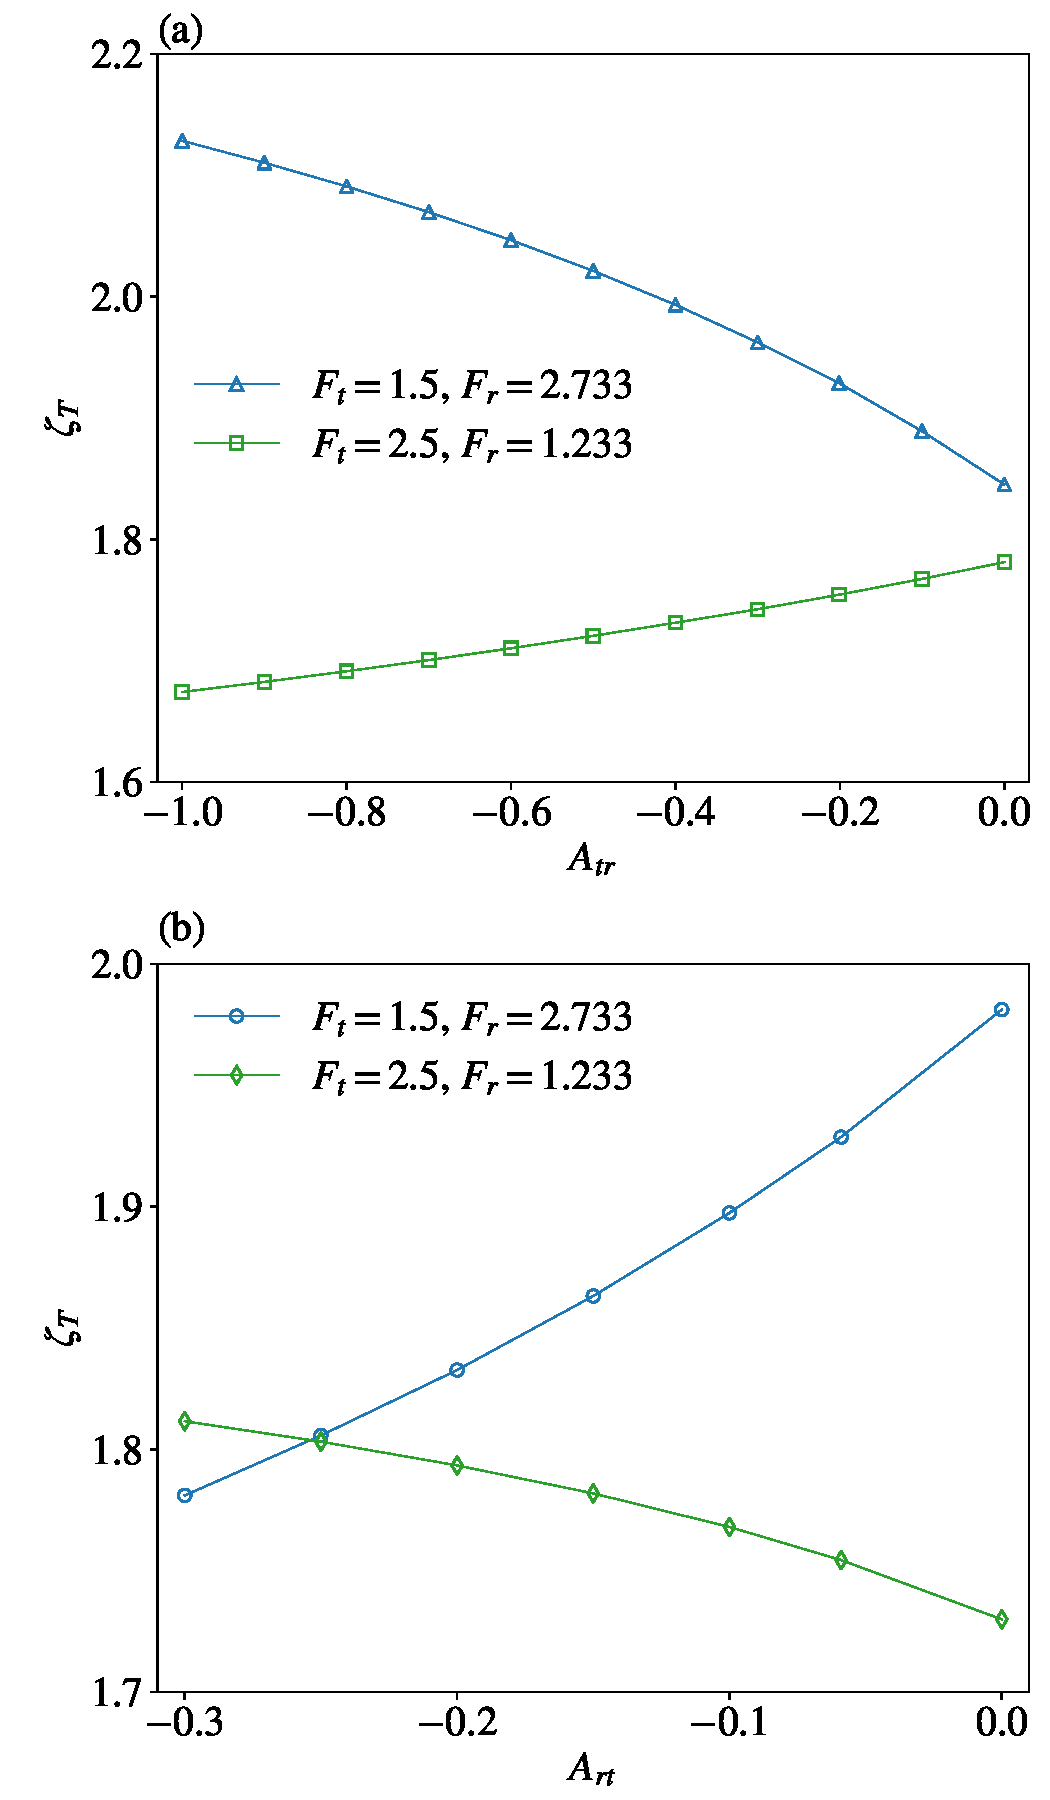
\includegraphics[width=0.4\columnwidth]{SlipJump/IMG/TJC_QtQr}%
	\caption{Temperature jump coefficient displaying the influence of the cross relaxation rates $A_{tr}$ and $A_{rt}$ when $Z=2.667$, $f_{u}=1.993$, while $f_{tr}$ and $f_{rot}$ are fixed: (a) $A_{tr}$ varies and $A_{rt}=-0.059$; (b) $A_{tr}=-0.201$ and $A_{rt}$ varies.}
	\label{fig:TJC_QtQr}
\end{figure}


